%%%%%%%%%%%%%%%%%%%%%%%%%%%%%%%%%%%%%%%%%%%%%%%%%%%%%%%%%%%%%%%%%%%%%%%%%%%%%%%%%%
\begin{frame}[fragile]\frametitle{}
\begin{center}
{\Large Concepts in AI Agents}

{\tiny (Ref: Vizuara AI Agents Bootcamp)}
\end{center}
\end{frame}

%%%%%%%%%%%%%%%%%%%%%%%%%%%%%%%%%%%%%%%%%%%%%%%%%%%%%%%%%%%
\begin{frame}[fragile]\frametitle{The Alien's Next Token Prediction Problem}

\begin{columns}
    \begin{column}[T]{0.6\linewidth}
      \begin{itemize}
	  \item Imagine an alien mathematician with access to all human data but no language knowledge
	  \item Task: Predict the next word in "Every effort moves you"
	  \item Simple approach: Find sequence occurrences and choose most frequent next word
	  \item Works for single token prediction using statistical frequency
	  \item Challenge emerges when predicting multiple tokens sequentially
	  \item Method breaks down for sequences not present in training dataset
	  \end{itemize}

    \end{column}
    \begin{column}[T]{0.4\linewidth}
		\begin{center}
		
\includegraphics[width=\linewidth,keepaspectratio]{aiagents46}

		{\tiny (Ref: Vizuara AI Agents Bootcamp)}

		\end{center}	
    \end{column}
  \end{columns}
  
\end{frame}

%%%%%%%%%%%%%%%%%%%%%%%%%%%%%%%%%%%%%%%%%%%%%%%%%%%%%%%%%%%
\begin{frame}[fragile]\frametitle{The Combinatorial Explosion Problem}
      \begin{itemize}
	  \item English language has approximately 40,000 words
	  \item Next token prediction: 40,000 possible choices
	  \item Next two tokens: 40,000 × 40,000 = 1.6 billion combinations
	  \item Next three tokens: 64 trillion possible combinations
	  \item Next twenty tokens: More combinations than particles in the universe
	  \item Statistical prediction becomes computationally impossible
	  \item Need new approach beyond simple frequency counting
	  \end{itemize}
\end{frame}

%%%%%%%%%%%%%%%%%%%%%%%%%%%%%%%%%%%%%%%%%%%%%%%%%%%%%%%%%%%
\begin{frame}[fragile]\frametitle{Learning from Galileo: The Power of Models}

\begin{columns}
    \begin{column}[T]{0.6\linewidth}
      \begin{itemize}
	  \item Galileo dropped objects from Leaning Tower of Pisa
	  \item Recorded experimental observations of fall times
	  \item Physicists convert observations into mathematical models
	  \item Models enable predictions beyond available experimental data
	  \item Can predict fall time for any height using the model
	  \item Models generalize from limited data to unlimited scenarios
	  \item Same principle applies to language prediction problems
	  \end{itemize}

    \end{column}
    \begin{column}[T]{0.4\linewidth}
		\begin{center}
		
\includegraphics[width=\linewidth,keepaspectratio]{aiagents45}

		{\tiny (Ref: Vizuara AI Agents Bootcamp)}

		\end{center}	
    \end{column}
  \end{columns}
  
 
\end{frame}

%%%%%%%%%%%%%%%%%%%%%%%%%%%%%%%%%%%%%%%%%%%%%%%%%%%%%%%%%%%
\begin{frame}[fragile]\frametitle{Introduction to Large Language Models}

\begin{columns}
    \begin{column}[T]{0.6\linewidth}
      \begin{itemize}
	  \item LLMs solve the alien's problem using modeling approach
	  \item Take sequence of words as input, output next token prediction
	  \item Can be used recursively to predict any number of words
	  \item Work even when input sequence not present in training data
	  \item Generate coherent text through learned language patterns
	  \item Represent breakthrough in natural language processing
	  \item Enable generalization beyond simple statistical lookup
	  \end{itemize}

    \end{column}
    \begin{column}[T]{0.4\linewidth}
		\begin{center}
		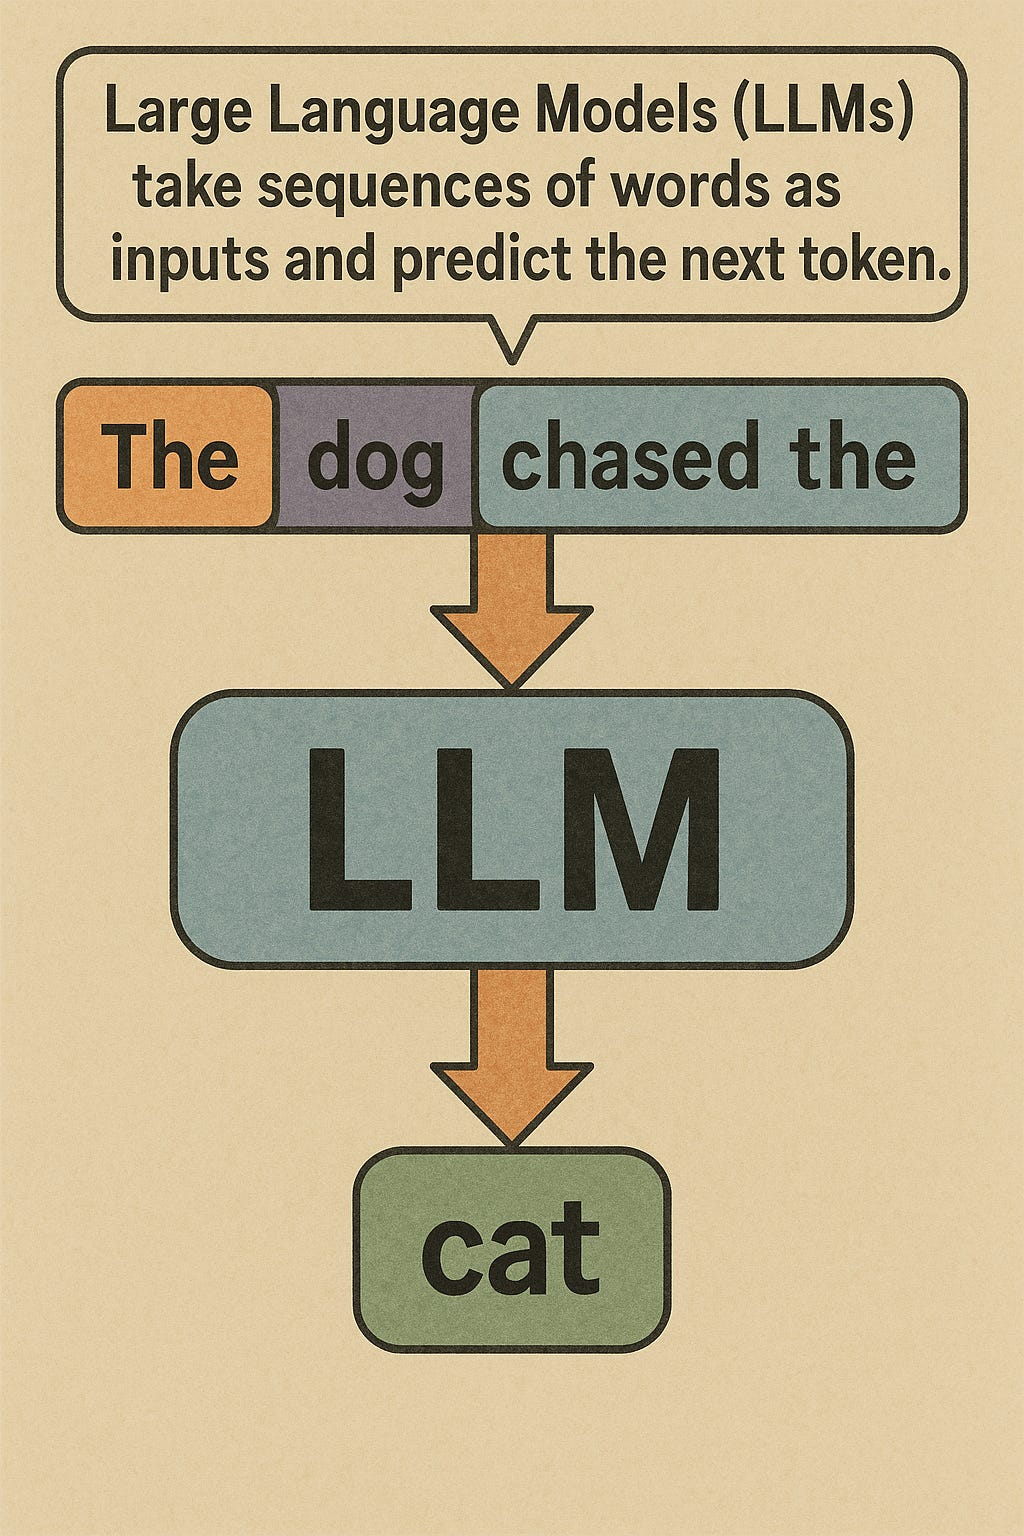
\includegraphics[width=\linewidth,keepaspectratio]{aiagents44}

		{\tiny (Ref: Vizuara AI Agents Bootcamp)}

		\end{center}	
    \end{column}
  \end{columns}
	  
\end{frame}

%%%%%%%%%%%%%%%%%%%%%%%%%%%%%%%%%%%%%%%%%%%%%%%%%%%%%%%%%%%
\begin{frame}[fragile]\frametitle{What Makes Language Models "Large"?}
      \begin{itemize}
	  \item "Large" refers to enormous number of parameters
	  \item Linear models: 2 free parameters
	  \item Quadratic models: 3 free parameters
	  \item Large Language Models: Billions of free parameters
	  \item GPT-3 largest model: 175 billion parameters
	  \item Simple definition: Next token prediction engines with billions of parameters
	  \item Scale enables complex pattern recognition and generation
	  \end{itemize}
		\begin{center}
		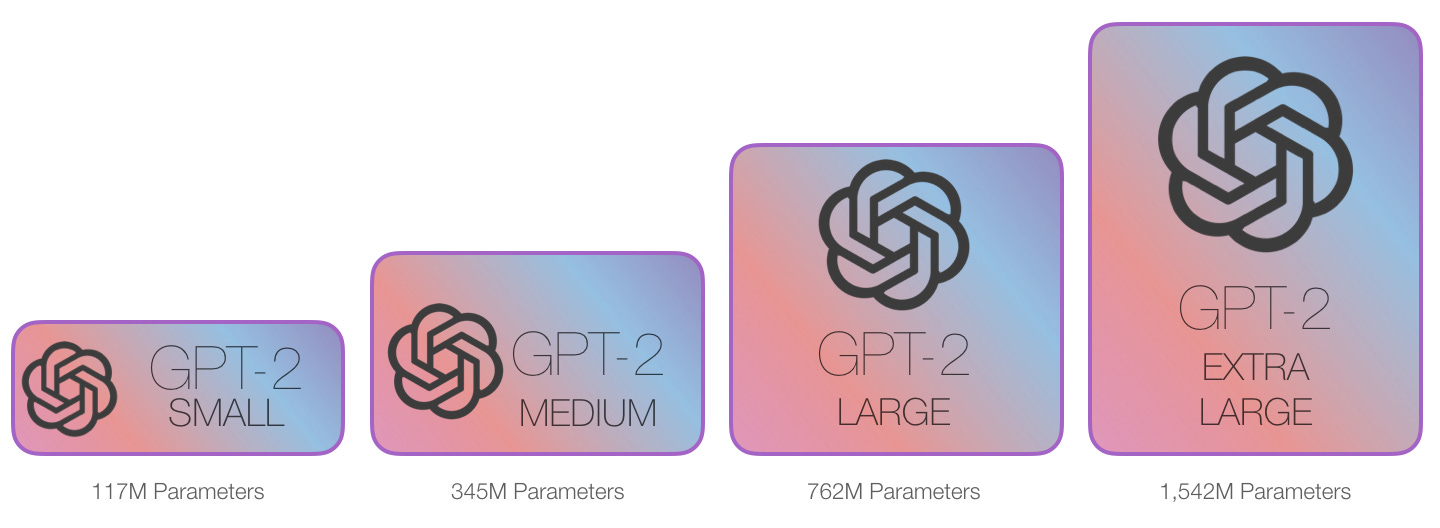
\includegraphics[width=0.8\linewidth,keepaspectratio]{aiagents43}

		{\tiny (Ref: Vizuara AI Agents Bootcamp)}

		\end{center}		  
\end{frame}

%%%%%%%%%%%%%%%%%%%%%%%%%%%%%%%%%%%%%%%%%%%%%%%%%%%%%%%%%%%
\begin{frame}[fragile]\frametitle{Why Size Matters: Emergent Abilities}
      \begin{itemize}
	  \item LLMs exhibit emergent abilities as they scale up
	  \item Emergent ability: Not present in smaller models, appears in larger ones
	  \item Performance suddenly improves after crossing size threshold
	  \item Many language tasks show dramatic improvement with scale
	  \item Drives push for increasingly larger model architectures
	  \item Size enables qualitatively different capabilities
	  \item Threshold effects create step-function improvements
	  \end{itemize}
	  
		\begin{center}
		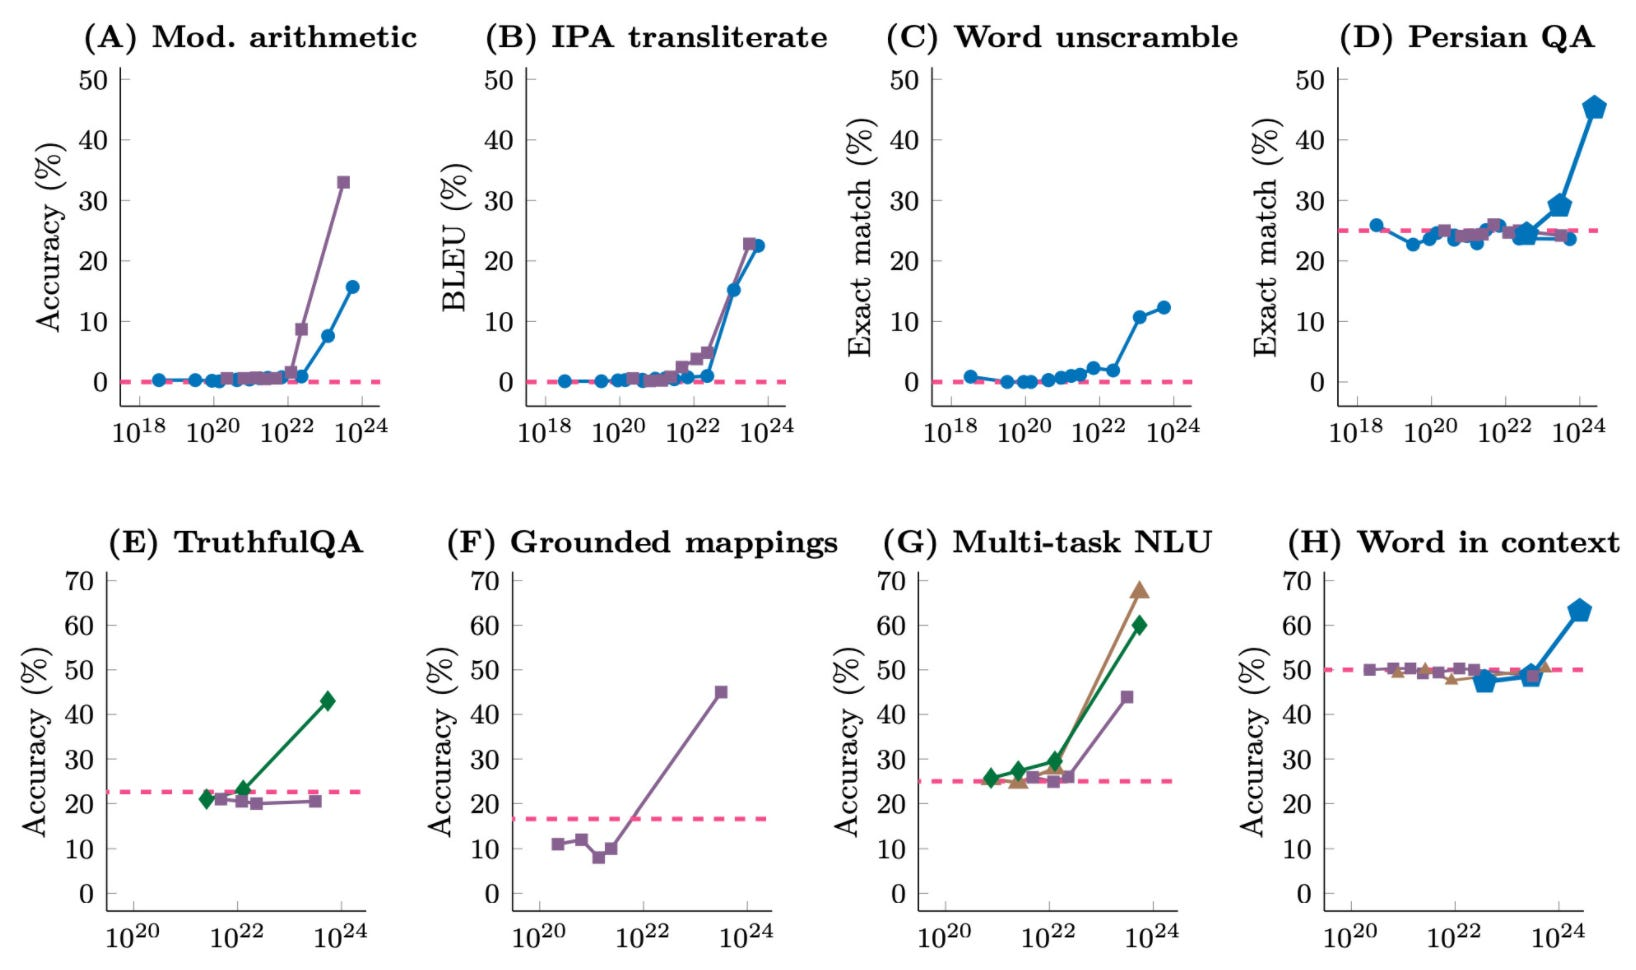
\includegraphics[width=0.6\linewidth,keepaspectratio]{aiagents41}

		{\tiny (Ref: Vizuara AI Agents Bootcamp)}

		\end{center}	  
\end{frame}

%%%%%%%%%%%%%%%%%%%%%%%%%%%%%%%%%%%%%%%%%%%%%%%%%%%%%%%%%%%
\begin{frame}[fragile]\frametitle{How Models Learn Language Through Next Token Prediction}
      \begin{itemize}
	  \item Models trained only on next token prediction task
	  \item Discover that learning language itself is most efficient strategy
	  \item Language encompasses both form and meaning
	  \item Models learn grammar, syntax, semantics, and world knowledge
	  \item Complex task requires millions of parameters to execute effectively
	  \item Emergent understanding arises from prediction objective
	  \item Language learning complexity justifies massive parameter counts
	  \end{itemize}
	  
		\begin{center}
		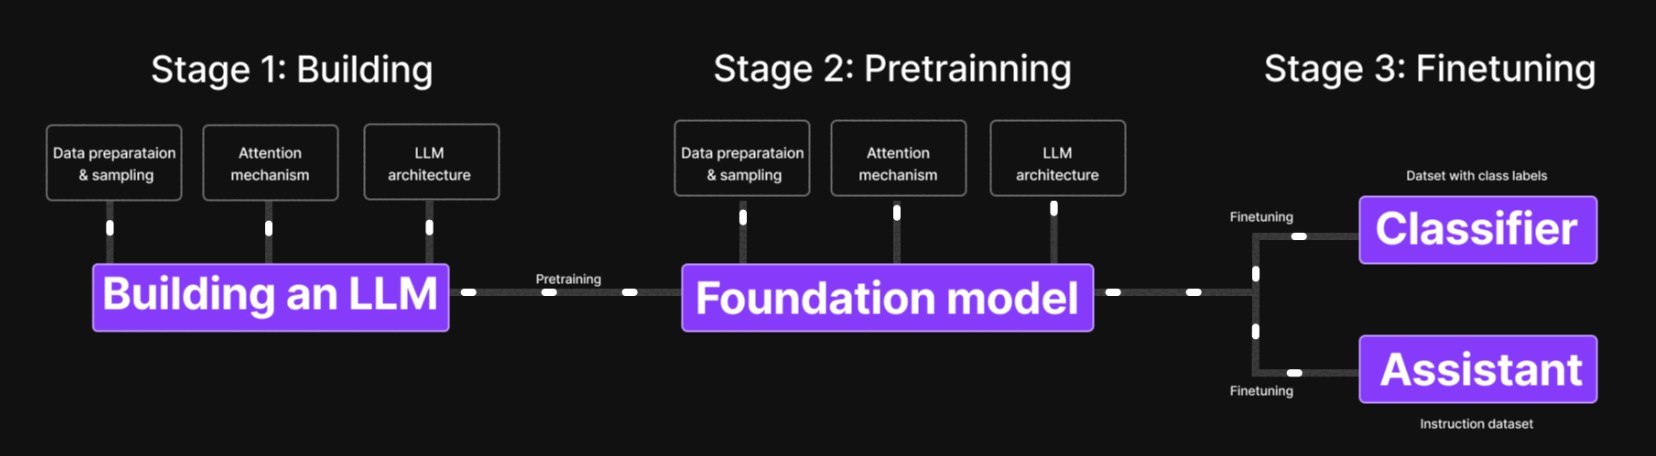
\includegraphics[width=0.8\linewidth,keepaspectratio]{aiagents42}

		{\tiny (Ref: Vizuara AI Agents Bootcamp)}

		\end{center}		  
\end{frame}

%%%%%%%%%%%%%%%%%%%%%%%%%%%%%%%%%%%%%%%%%%%%%%%%%%%%%%%%%%%
\begin{frame}[fragile]\frametitle{Pre-training: Foundation Building}
      \begin{itemize}
	  \item Most computationally intensive phase of LLM development
	  \item Exposed to massive corpus of unlabeled text data
	  \item Data sources: web pages, books, articles, diverse domains
	  \item Goal: Learn statistical patterns of language through next-token prediction
	  \item Learns grammar, syntax, word associations, and factual knowledge
	  \item Attention mechanism enables contextual relationship learning
	  \item Results in foundation model with general language capabilities
	  \item Not yet optimized for specific downstream tasks
	  \end{itemize}
\end{frame}

%%%%%%%%%%%%%%%%%%%%%%%%%%%%%%%%%%%%%%%%%%%%%%%%%%%%%%%%%%%
\begin{frame}[fragile]\frametitle{Fine-tuning: Specialization and Application}
      \begin{itemize}
	  \item Adapts pre-trained foundation model for specific tasks
	  \item Uses curated, task-specific datasets instead of general data
	  \item Examples: sentiment classification, conversational assistance
	  \item Instruction-tuned datasets teach following human instructions
	  \item Minor weight adjustments preserve broad capabilities while specializing
	  \item Creates practical applications: chatbots, summarizers, report generators
	  \item Transforms general foundation model into targeted tools
	  \item Enables deployment for specific use cases and domains
	  \end{itemize}
\end{frame}

%%%%%%%%%%%%%%%%%%%%%%%%%%%%%%%%%%%%%%%%%%%%%%%%%%%%%%%%%%%%%%%%%%%%%%%%%%%%%%%%%%
\begin{frame}[fragile]\frametitle{}
\begin{center}
{\Large Components}
\end{center}
\end{frame}

%%%%%%%%%%%%%%%%%%%%%%%%%%%%%%%%%%%%%%%%%%%%%%%%%%%%%%%%%%%
\begin{frame}[fragile]\frametitle{Planning and Reasoning}

      \begin{itemize}
        \item Planning breaks tasks into executable steps.
        \item Requires reasoning before taking action.
        \item Enabled via few-shot prompting or fine-tuning.
        \item Chain-of-Thought prompts guide structured thinking.
        \item ReAct combines reasoning with tool use.
        \item Reflexion and SELF-REFINE add self-feedback loops.
        \item Reflective loops improve task accuracy over time.
      \end{itemize}

\end{frame}

%%%%%%%%%%%%%%%%%%%%%%%%%%%%%%%%%%%%%%%%%%%%%%%%%%%%%%%%%%%%%%%%%%%%%%%%%%%%%%%%%%
\begin{frame}[fragile]\frametitle{}
\begin{center}
{\Large Tools}
\end{center}
\end{frame}

%%%%%%%%%%%%%%%%%%%%%%%%%%%%%%%%%%%%%%%%%%%%%%%%%%%%%%%%%%%%%%%%%%%%%%%%%%%%%%%%%%
\begin{frame}[fragile]\frametitle{Tool Use in LLM Agents}

      \begin{itemize}
        \item Tools help LLMs fetch data or perform actions.
        \item Tools are accessed via prompts or function calls.
        \item JSON-format is commonly used for tool instructions.
        \item Toolformer trained LLMs to decide API usage via tokens.
        \item LLMs can be fine-tuned for robust tool use.
        \item Tools may be statically ordered or selected autonomously.
        \item Intermediate outputs can loop back into the LLM.
        \item More tools = stronger Agentic capabilities.
      \end{itemize}

\end{frame}

%%%%%%%%%%%%%%%%%%%%%%%%%%%%%%%%%%%%%%%%%%%%%%%%%%%%%%%%%%%%%%%%%%%%%%%%%%%%%%%%%%
\begin{frame}[fragile]\frametitle{Tools in LLM Agents}

        \begin{center}
        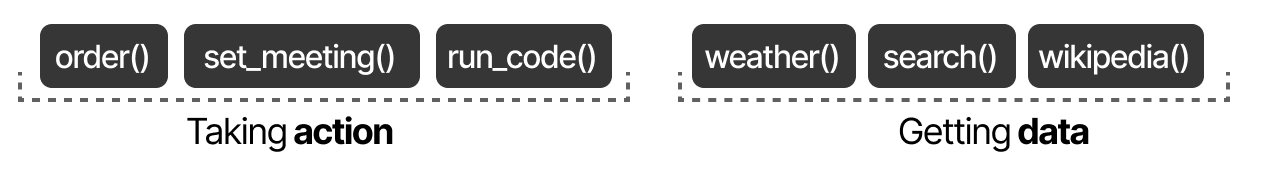
\includegraphics[width=0.8\linewidth,keepaspectratio]{aiagents110}

        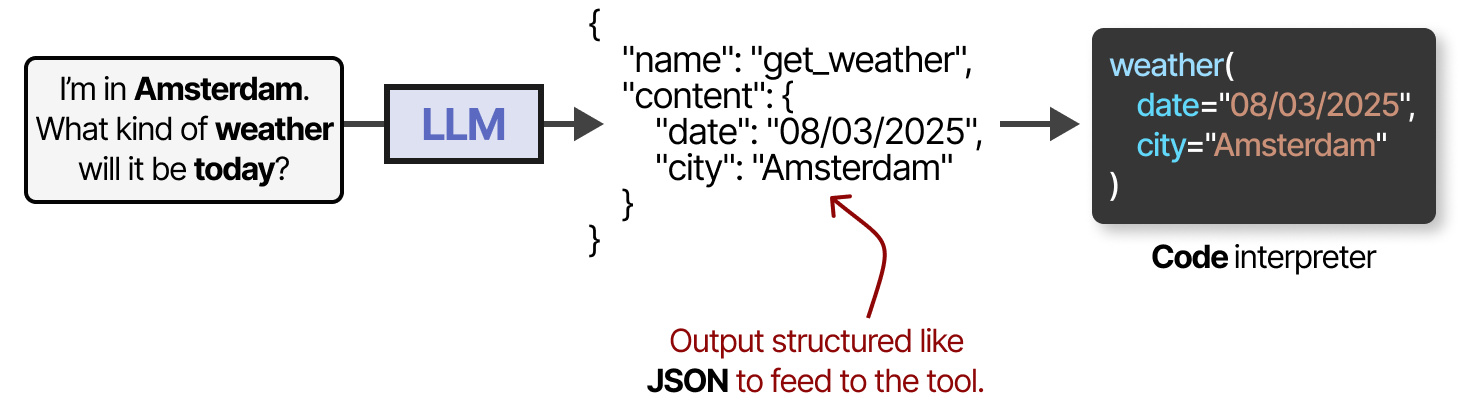
\includegraphics[width=0.8\linewidth,keepaspectratio]{aiagents111}
		
        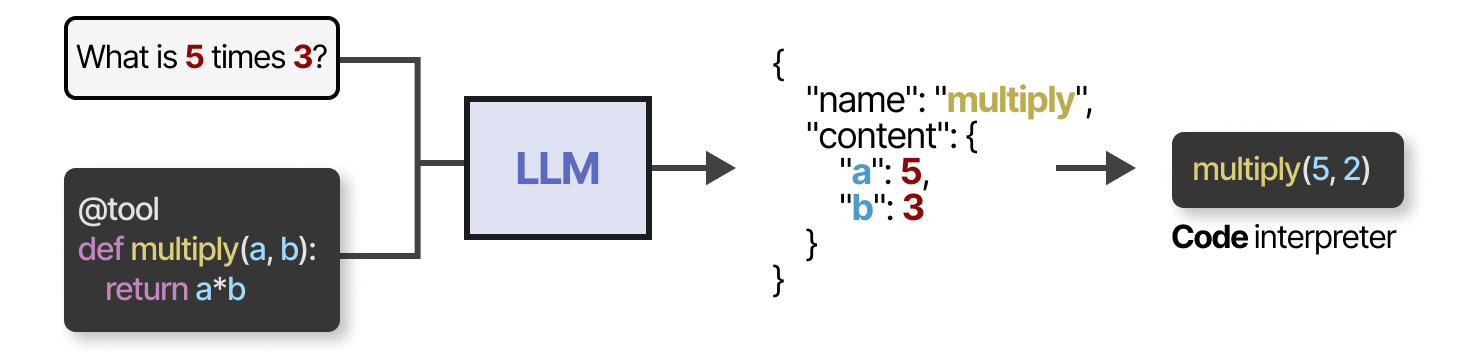
\includegraphics[width=0.8\linewidth,keepaspectratio]{aiagents112}

		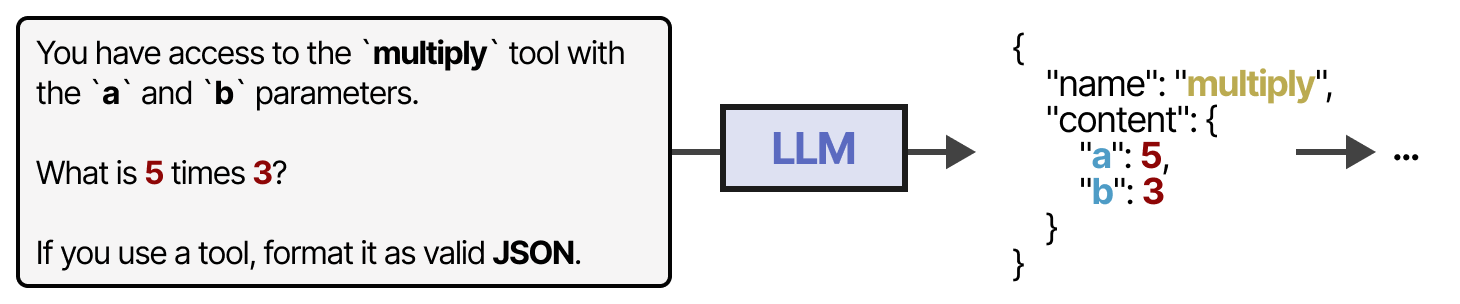
\includegraphics[width=0.8\linewidth,keepaspectratio]{aiagents113}

        {\tiny (Ref: A Visual Guide to Reasoning LLMs - Maarten Grootendorst)}
        \end{center}


\end{frame}

%%%%%%%%%%%%%%%%%%%%%%%%%%%%%%%%%%%%%%%%%%%%%%%%%%%%%%%%%%%%%%%%%%%%%%%%%%%%%%%%%%
\begin{frame}[fragile]\frametitle{Tools in LLM Agents}

        \begin{center}
		
        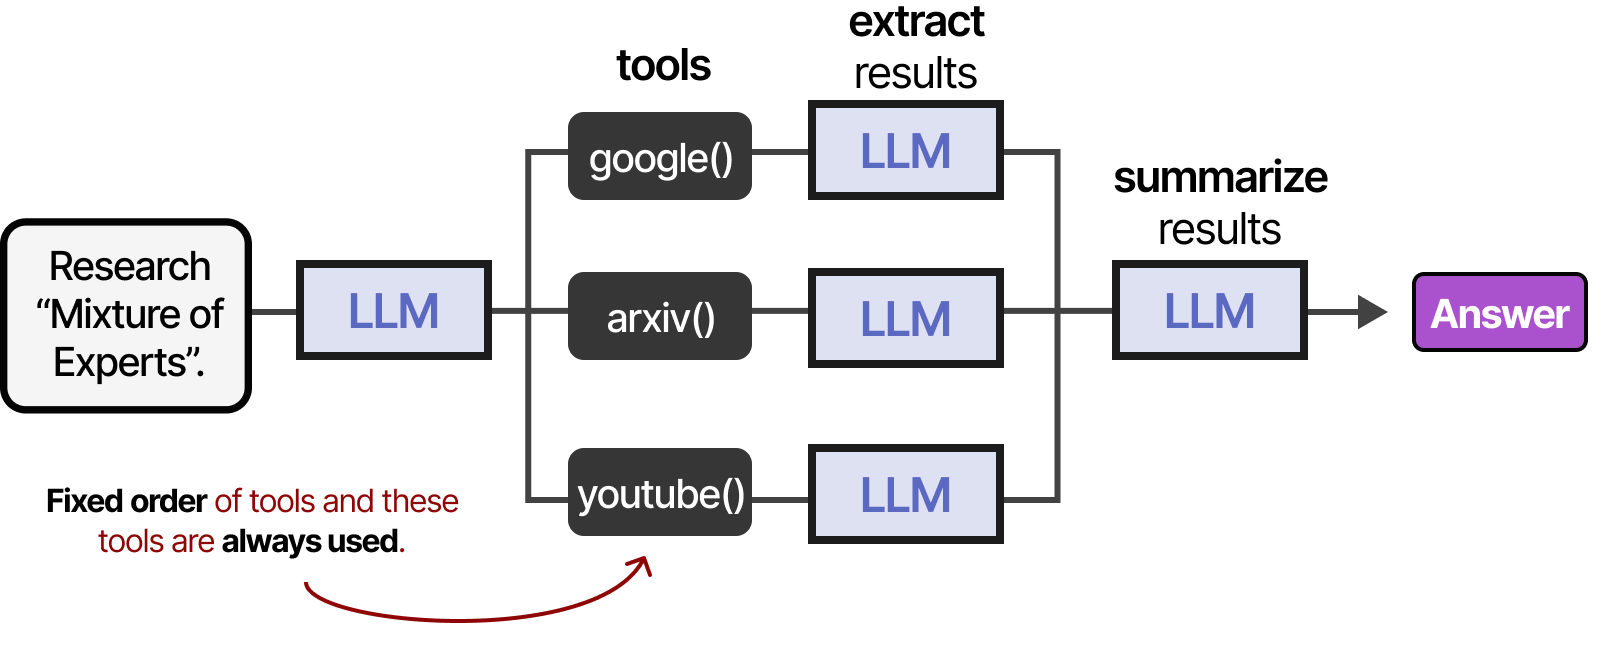
\includegraphics[width=0.8\linewidth,keepaspectratio]{aiagents114}

		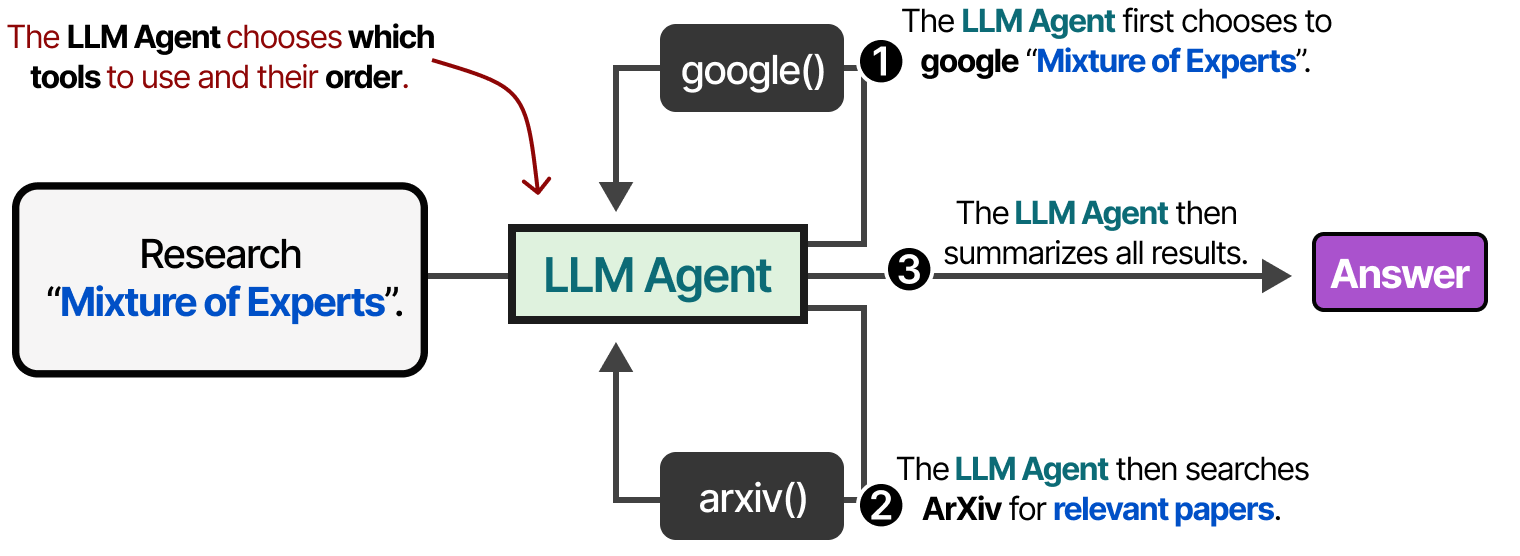
\includegraphics[width=0.8\linewidth,keepaspectratio]{aiagents115}
		
		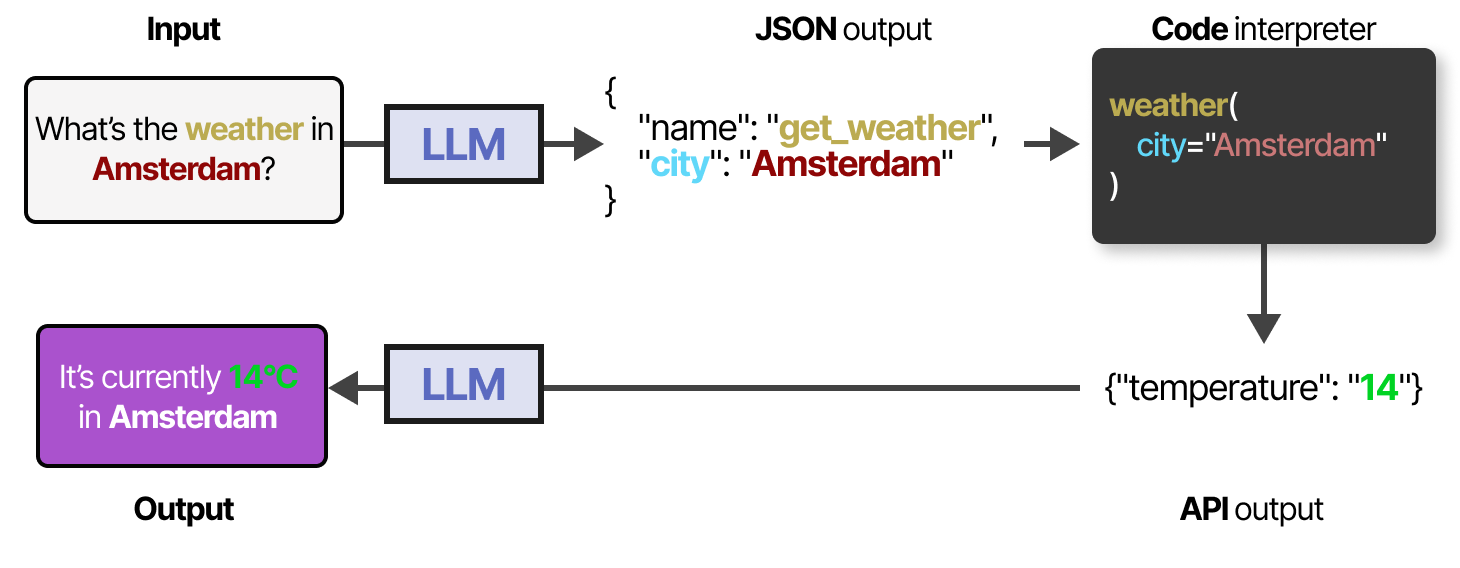
\includegraphics[width=0.8\linewidth,keepaspectratio]{aiagents116}
		

        {\tiny (Ref: A Visual Guide to Reasoning LLMs - Maarten Grootendorst)}
        \end{center}


\end{frame}

%%%%%%%%%%%%%%%%%%%%%%%%%%%%%%%%%%%%%%%%%%%%%%%%%%%%%%%%%%%
\begin{frame}[fragile]\frametitle{What Are Tools in Agentic AI?}
      \begin{itemize}
        \item Tools are external capabilities the LLM can call
        \item Examples: APIs, database queries, services, internal functions
        \item Transform LLMs from passive responders to active agents
        \item Enable real-time access and action
        \item Core to execution, not just generation
      \end{itemize}
\end{frame}

%%%%%%%%%%%%%%%%%%%%%%%%%%%%%%%%%%%%%%%%%%%%%%%%%%%%%%%%%%%
\begin{frame}[fragile]\frametitle{Why Tools Matter}
      \begin{itemize}
        \item Unlock full workflow execution, not just suggestions
        \item Increase precision by avoiding hallucination
        \item Define boundaries to control risk and exposure
        \item Enable composability across systems (CRM, calendar, etc.)
      \end{itemize}
\end{frame}

%%%%%%%%%%%%%%%%%%%%%%%%%%%%%%%%%%%%%%%%%%%%%%%%%%%%%%%%%%%
\begin{frame}[fragile]\frametitle{Tools in Action: Example Workflow}
      \begin{itemize}
        \item Input: ``Let John know his order is delayed and reschedule''
        \item LLM plans steps: check status, find slot, email, log
        \item Calls tools: \lstinline|get_order_status(), get_available_slots()|, etc.
        \item Generates message and triggers execution
        \item Logs events and updates systems
      \end{itemize}
	  
		\begin{center}
		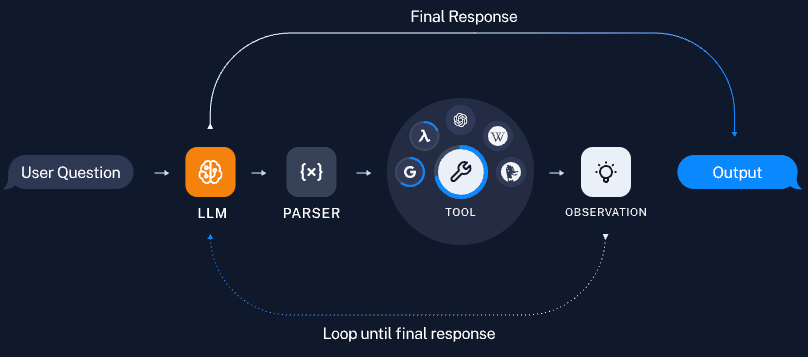
\includegraphics[width=\linewidth,keepaspectratio]{aiagents18}
		
		{\tiny (Ref: Agentic AI For Everyone - Aish \& Kiriti)}
		\end{center}	  
\end{frame}

%%%%%%%%%%%%%%%%%%%%%%%%%%%%%%%%%%%%%%%%%%%%%%%%%%%%%%%%%%%
\begin{frame}[fragile]\frametitle{How the Tool Loop Works}
      \begin{itemize}
        \item User gives task; LLM plans next step
        \item Parser converts text to structured tool call
        \item Tool is executed externally and returns a result
        \item LLM uses result to plan the next action
        \item Loop continues until task is complete
      \end{itemize}
\end{frame}

%%%%%%%%%%%%%%%%%%%%%%%%%%%%%%%%%%%%%%%%%%%%%%%%%%%%%%%%%%%
\begin{frame}[fragile]\frametitle{Agent Loop: Reasoning to Action}
      \begin{itemize}
        \item LLM generates structured output (e.g., JSON or function call)
        \item System executes it and feeds back the observation
        \item LLM reflects and adjusts next step
        \item Loop of plan → act → observe → repeat
        \item Powering modern agents in LangChain, CrewAI, AutoGen, etc.
      \end{itemize}
\end{frame}

%%%%%%%%%%%%%%%%%%%%%%%%%%%%%%%%%%%%%%%%%%%%%%%%%%%%%%%%%%%
\begin{frame}[fragile]\frametitle{What Makes a Tool Usable}
      \begin{itemize}
        \item Each tool needs: name, description, input/output schema
        \item Metadata lets the LLM reason when and how to use it
        \item Structured inputs allow reliable execution
        \item Structured outputs enable next-step reasoning
      \end{itemize}
\end{frame}

%%%%%%%%%%%%%%%%%%%%%%%%%%%%%%%%%%%%%%%%%%%%%%%%%%%%%%%%%%%
\begin{frame}[fragile]\frametitle{Structured I/O and Parsing}
      \begin{itemize}
        \item Parsers convert LLM output into executable tool calls
        \item Newer LLMs can output structured data directly
        \item JSON, function calls, or APIs simplify orchestration
        \item Structure makes loops robust and production-ready
      \end{itemize}
\end{frame}

%%%%%%%%%%%%%%%%%%%%%%%%%%%%%%%%%%%%%%%%%%%%%%%%%%%%%%%%%%%
\begin{frame}[fragile]\frametitle{The Bottom Line}
      \begin{itemize}
        \item LLMs alone can understand and generate text
        \item With tools, they can observe and act
        \item This turns passive models into powerful agents
        \item Tools bridge understanding and execution
      \end{itemize}
\end{frame}

%%%%%%%%%%%%%%%%%%%%%%%%%%%%%%%%%%%%%%%%%%%%%%%%%%%%%%%%%%%%%%%%%%%%%%%%%%%%%%%%%%
\begin{frame}[fragile]\frametitle{}
\begin{center}
{\Large Memory}

{\tiny (Ref: AI Agents - Aish \& Kiriti)}
\end{center}
\end{frame}

%%%%%%%%%%%%%%%%%%%%%%%%%%%%%%%%%%%%%%%%%%%%%%%%%%%%%%%%%%%%%%%%%%%%%%%%%%%%%%%%%%
\begin{frame}[fragile]\frametitle{Memory in LLM Agents}

      \begin{itemize}
        \item LLMs lack built-in memory—context is key.
        \item Short-term memory: use context window or summaries.
        \item Long-term memory: store embeddings in vector databases.
        \item Retrieval-Augmented Generation (RAG) fetches past info.
        \item External memory allows tracking past actions and sessions.
        \item Different memory types map to different cognitive functions.
        \item Semantic, working, and episodic memory can be separated.
      \end{itemize}

\end{frame}


%%%%%%%%%%%%%%%%%%%%%%%%%%%%%%%%%%%%%%%%%%%%%%%%%%%%%%%%%%%%%%%%%%%%%%%%%%%%%%%%%%
\begin{frame}[fragile]\frametitle{Memory in LLM Agents}


\begin{columns}
    \begin{column}[T]{0.6\linewidth}
        \begin{center}
        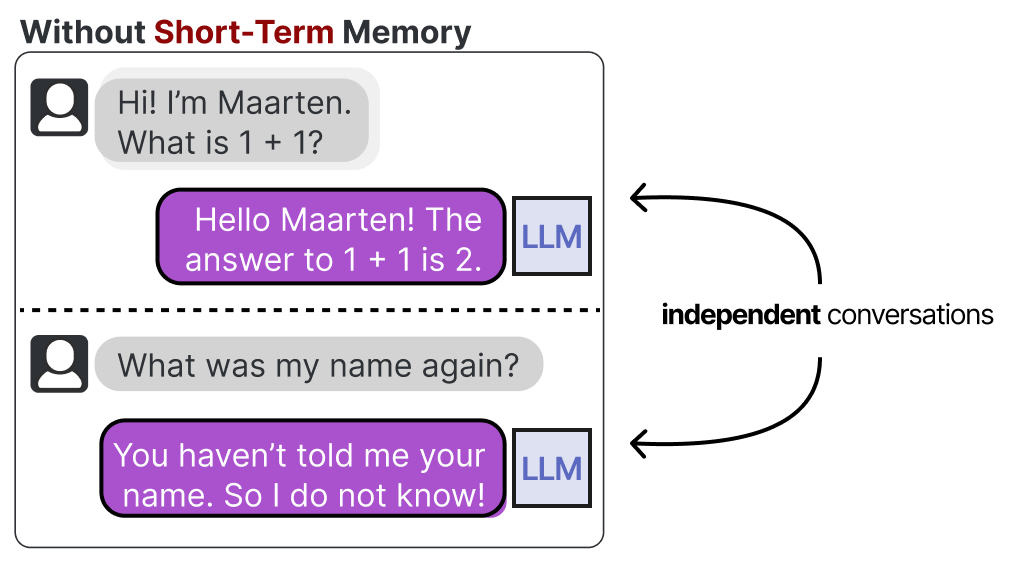
\includegraphics[width=0.8\linewidth,keepaspectratio]{aiagents101}

		
        {\tiny (Ref: A Visual Guide to Reasoning LLMs - Maarten Grootendorst)}
        \end{center}

    \end{column}
    \begin{column}[T]{0.4\linewidth}
        \begin{center}
        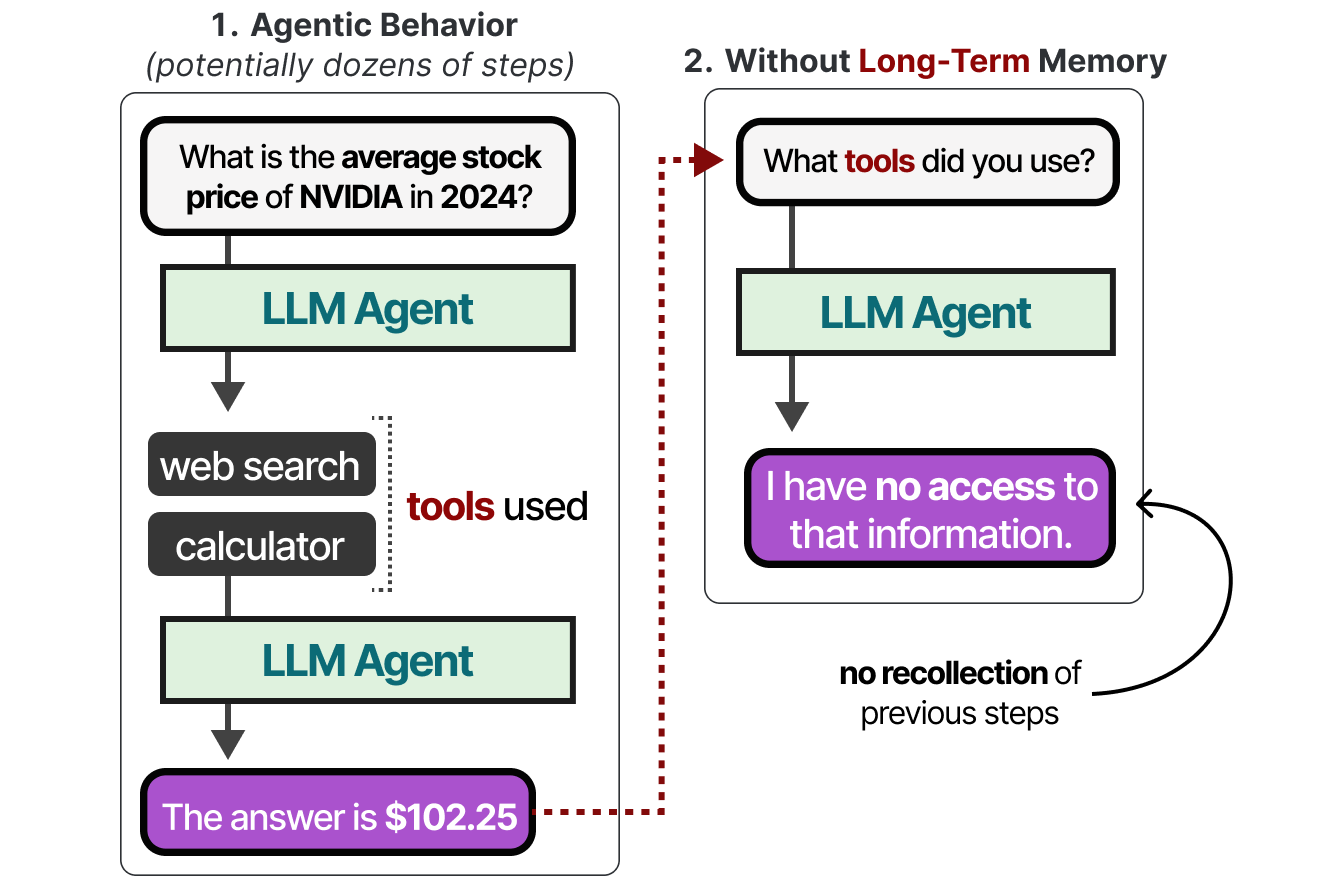
\includegraphics[width=0.8\linewidth,keepaspectratio]{aiagents102}

		
        {\tiny (Ref: A Visual Guide to Reasoning LLMs - Maarten Grootendorst)}
        \end{center}
    \end{column}
  \end{columns}

\end{frame}

%%%%%%%%%%%%%%%%%%%%%%%%%%%%%%%%%%%%%%%%%%%%%%%%%%%%%%%%%%%%%%%%%%%%%%%%%%%%%%%%%%
\begin{frame}[fragile]\frametitle{Memory in LLM Agents}

        \begin{center}
        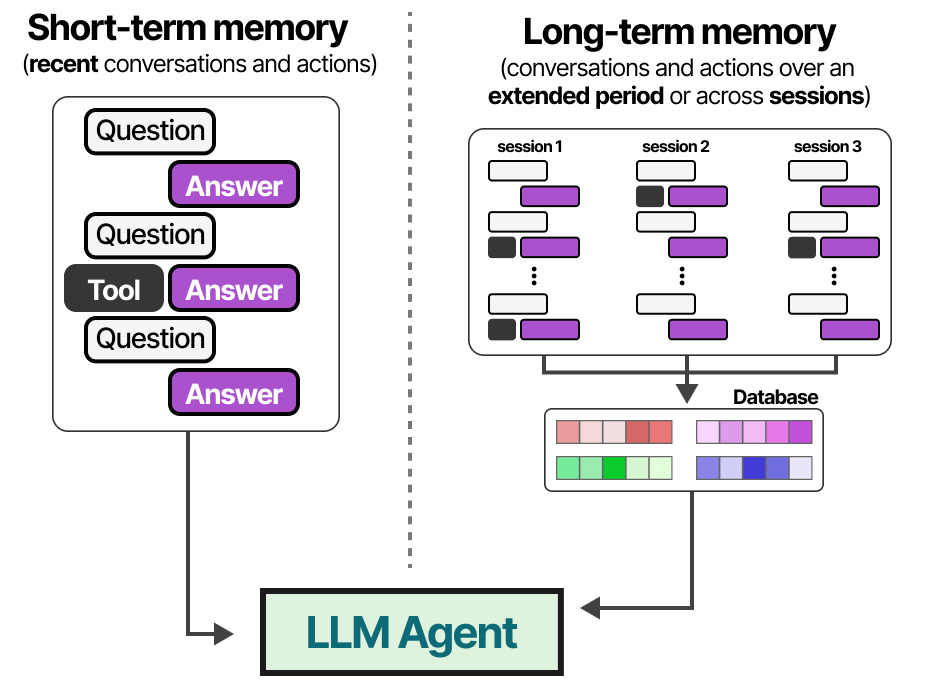
\includegraphics[width=0.8\linewidth,keepaspectratio]{aiagents103}

		
        {\tiny (Ref: A Visual Guide to Reasoning LLMs - Maarten Grootendorst)}
        \end{center}


\end{frame}

%%%%%%%%%%%%%%%%%%%%%%%%%%%%%%%%%%%%%%%%%%%%%%%%%%%%%%%%%%%%%%%%%%%%%%%%%%%%%%%%%%
\begin{frame}[fragile]\frametitle{Short Term Memory in LLM Agents}


\begin{columns}
    \begin{column}[T]{0.6\linewidth}
        \begin{center}
        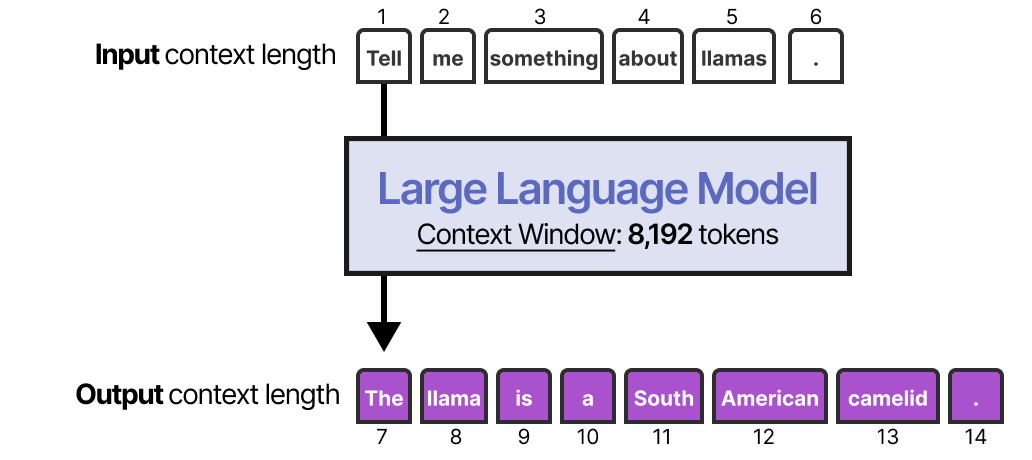
\includegraphics[width=0.8\linewidth,keepaspectratio]{aiagents104}

		
        {\tiny (Ref: A Visual Guide to Reasoning LLMs - Maarten Grootendorst)}
        \end{center}

    \end{column}
    \begin{column}[T]{0.4\linewidth}
        \begin{center}
        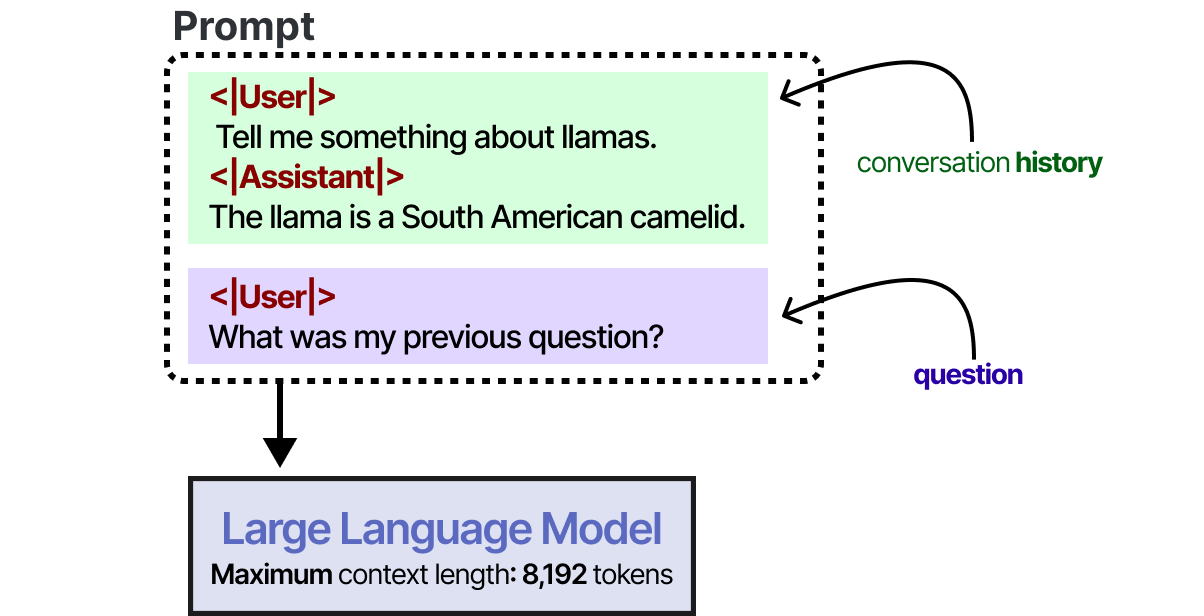
\includegraphics[width=0.8\linewidth,keepaspectratio]{aiagents105}

		
        {\tiny (Ref: A Visual Guide to Reasoning LLMs - Maarten Grootendorst)}
        \end{center}
    \end{column}
  \end{columns}

\end{frame}

%%%%%%%%%%%%%%%%%%%%%%%%%%%%%%%%%%%%%%%%%%%%%%%%%%%%%%%%%%%%%%%%%%%%%%%%%%%%%%%%%%
\begin{frame}[fragile]\frametitle{Short Term Memory in LLM Agents}



        \begin{center}
        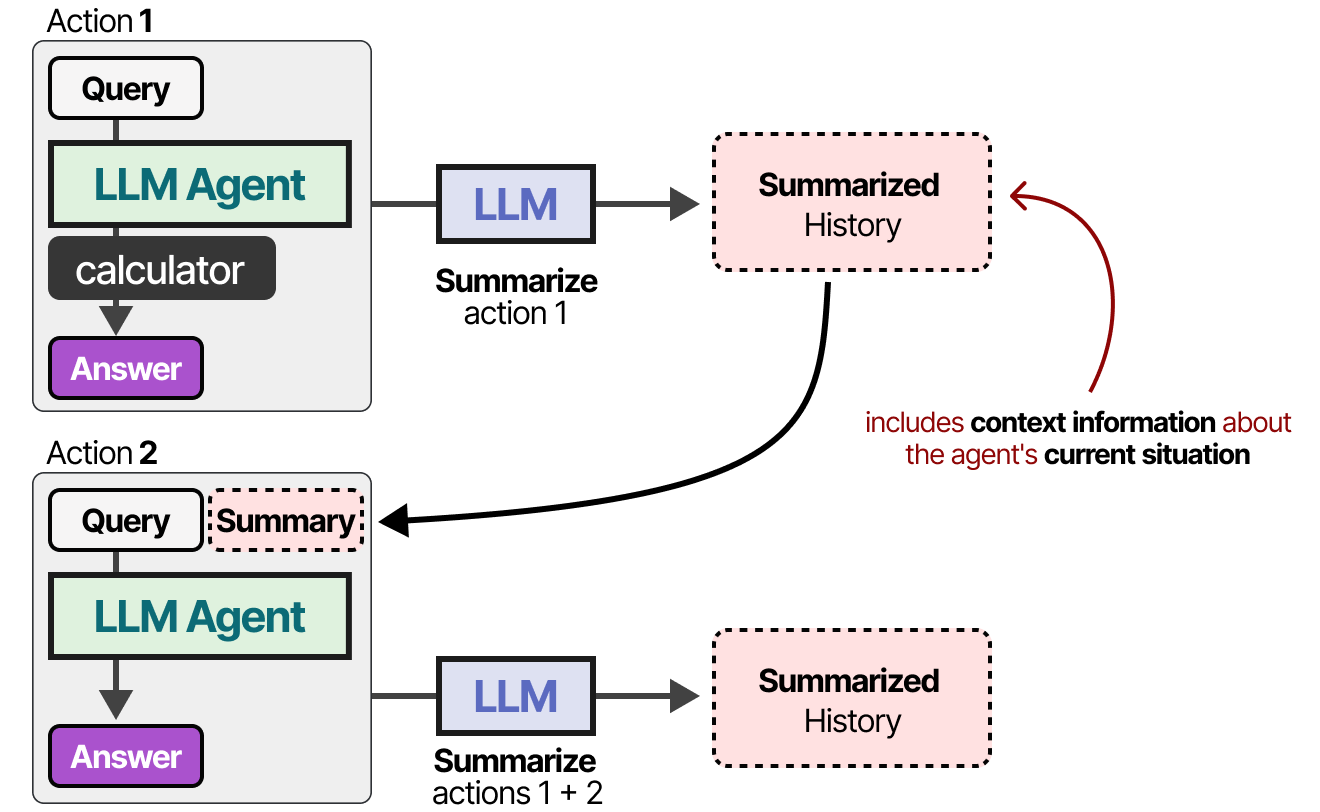
\includegraphics[width=0.8\linewidth,keepaspectratio]{aiagents106}

		
        {\tiny (Ref: A Visual Guide to Reasoning LLMs - Maarten Grootendorst)}
        \end{center}

\end{frame}

%%%%%%%%%%%%%%%%%%%%%%%%%%%%%%%%%%%%%%%%%%%%%%%%%%%%%%%%%%%%%%%%%%%%%%%%%%%%%%%%%%
\begin{frame}[fragile]\frametitle{Long Term Memory in LLM Agents}



        \begin{center}
        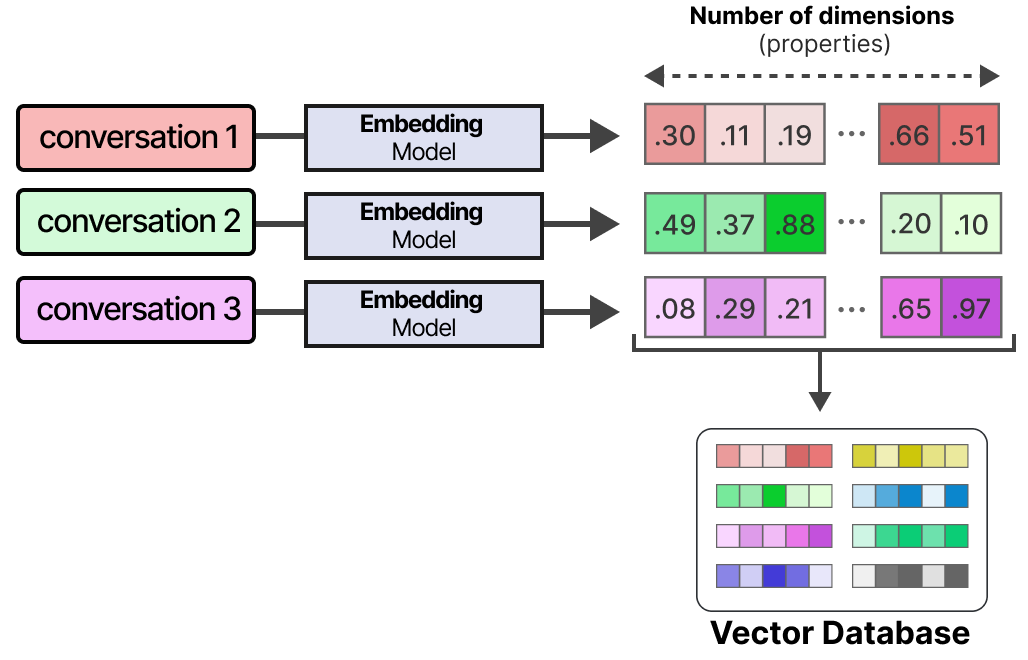
\includegraphics[width=0.8\linewidth,keepaspectratio]{aiagents107}

		
        {\tiny (Ref: A Visual Guide to Reasoning LLMs - Maarten Grootendorst)}
        \end{center}

\end{frame}

%%%%%%%%%%%%%%%%%%%%%%%%%%%%%%%%%%%%%%%%%%%%%%%%%%%%%%%%%%%%%%%%%%%%%%%%%%%%%%%%%%
\begin{frame}[fragile]\frametitle{Long Term Memory in LLM Agents}



        \begin{center}
        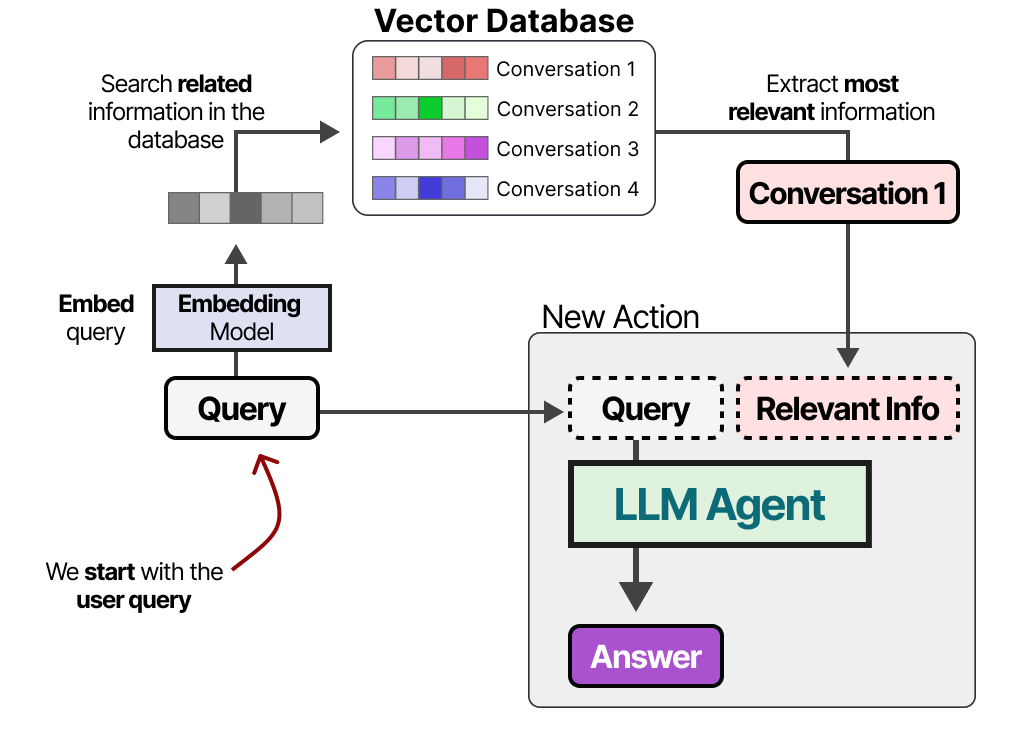
\includegraphics[width=0.8\linewidth,keepaspectratio]{aiagents108}

		
        {\tiny (Ref: A Visual Guide to Reasoning LLMs - Maarten Grootendorst)}
        \end{center}

\end{frame}

%%%%%%%%%%%%%%%%%%%%%%%%%%%%%%%%%%%%%%%%%%%%%%%%%%%%%%%%%%%%%%%%%%%%%%%%%%%%%%%%%%
\begin{frame}[fragile]\frametitle{Long Term Memory in LLM Agents}



        \begin{center}
        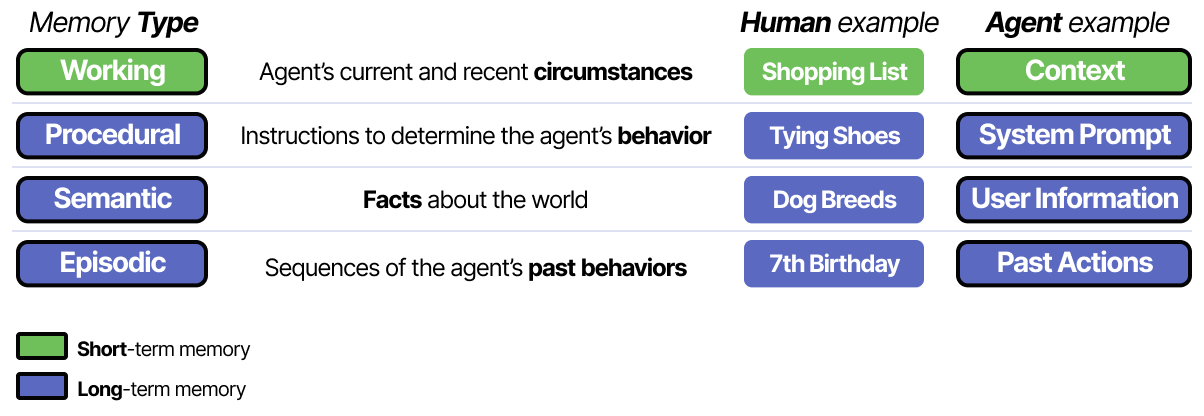
\includegraphics[width=0.8\linewidth,keepaspectratio]{aiagents109}

		
        {\tiny (Ref: A Visual Guide to Reasoning LLMs - Maarten Grootendorst)}
        \end{center}

\end{frame}

%%%%%%%%%%%%%%%%%%%%%%%%%%%%%%%%%%%%%%%%%%%%%%%%%%%%%%%%%%%
\begin{frame}[fragile]\frametitle{Why Memory Matters in AI Agents}
\begin{itemize}
  \item AI models are stateless by default.
  \item Each prompt is treated independently unless memory is added.
  \item Memory enables context retention across tasks and sessions.
  \item Useful for drafting emails, managing workflows, and personalization.
  \item Avoids re-passing the same info repeatedly.
  \item Allows agents to retrieve relevant context when needed.
  \item Memory $\neq$ RAG; intent differs despite similar mechanics.
  \item Memory supports coherent behavior over time.
\end{itemize}

\begin{center}
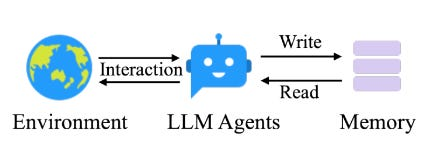
\includegraphics[width=0.8\linewidth,keepaspectratio]{aiagents19}

{\tiny (Ref: AI Agents - Aish \& Kiriti https://arxiv.org/html/2502.12110v1)}

\end{center}	
\end{frame}

%%%%%%%%%%%%%%%%%%%%%%%%%%%%%%%%%%%%%%%%%%%%%%%%%%%%%%%%%%%
\begin{frame}[fragile]\frametitle{How Memory Works in Agents}
\begin{itemize}
  \item Store structured/unstructured data with metadata or embeddings.
  \item Retrieve relevant memory slices at the right time.
  \item Ground model actions using retrieved context.
  \item Different from RAG which answers knowledge questions.
  \item Memory is about maintaining consistency, not just facts.
\end{itemize}
\end{frame}

%%%%%%%%%%%%%%%%%%%%%%%%%%%%%%%%%%%%%%%%%%%%%%%%%%%%%%%%%%%
\begin{frame}[fragile]\frametitle{Types of Memory in Agent Systems}

% \begin{columns}
    % \begin{column}[T]{0.6\linewidth}
		\begin{itemize}
		  \item Two main types: Short-term and Long-term memory.
		  \item Short-term: scoped to a single task or session.
		  \item Long-term: persists across days, weeks, or indefinitely.
		  \item Each serves different purposes and use cases.
		\end{itemize}

    % \end{column}
    % \begin{column}[T]{0.4\linewidth}
		\begin{center}
		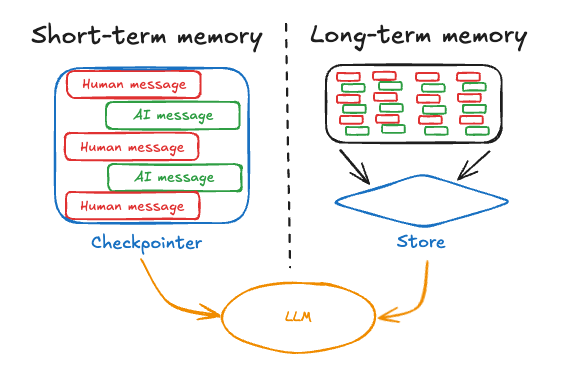
\includegraphics[width=0.7\linewidth,keepaspectratio]{aiagents20}

		{\tiny (Ref: AI Agents - Aish \& Kiriti https://langchain-ai.github.io/langgraph/concepts/memory/)}

		\end{center}
    % \end{column}
  % \end{columns}



\end{frame}

%%%%%%%%%%%%%%%%%%%%%%%%%%%%%%%%%%%%%%%%%%%%%%%%%%%%%%%%%%%
\begin{frame}[fragile]\frametitle{Short-Term Memory in Practice}
\begin{itemize}
  \item Includes conversation history, tool usage, and responses.
  \item Treated as part of agent "state" in frameworks like LangGraph.
  \item State grows fast—can hinder performance.
  \item Manage by trimming, summarizing, or filtering history.
  \item Balance context length vs relevance vs cost.
\end{itemize}
\end{frame}

%%%%%%%%%%%%%%%%%%%%%%%%%%%%%%%%%%%%%%%%%%%%%%%%%%%%%%%%%%%
\begin{frame}[fragile]\frametitle{Long-Term Memory: Persistent Context}
\begin{itemize}
  \item Helps agents remember user identity and preferences.
  \item Useful for continuity across sessions.
  \item Not about volume—retrieving the right info matters more.
  \item Enables consistent behavior and avoids redundant actions.
\end{itemize}
\end{frame}

%%%%%%%%%%%%%%%%%%%%%%%%%%%%%%%%%%%%%%%%%%%%%%%%%%%%%%%%%%%
\begin{frame}[fragile]\frametitle{Types of Long-Term Memory}


% \begin{columns}
    % \begin{column}[T]{0.6\linewidth}
		\begin{itemize}
		  \item Semantic Memory: Facts and user details.
		  \item Episodic Memory: Logs of past actions.
		  \item Procedural Memory: Preferences and behavior rules.
		  \item Inspired by cognitive science.
		  \item Each type serves different agent needs.
		\end{itemize}

    % \end{column}
    % \begin{column}[T]{0.4\linewidth}
		\begin{center}
		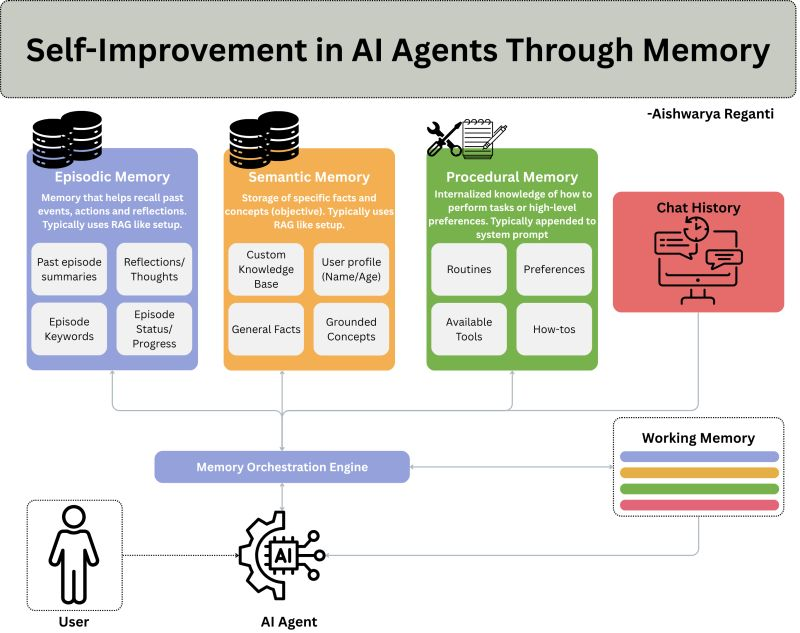
\includegraphics[width=0.5\linewidth,keepaspectratio]{aiagents21}

		{\tiny (Ref: AI Agents - Aish \& Kiriti)}

		\end{center}
    % \end{column}
  % \end{columns}
\end{frame}

%%%%%%%%%%%%%%%%%%%%%%%%%%%%%%%%%%%%%%%%%%%%%%%%%%%%%%%%%%%
\begin{frame}[fragile]\frametitle{Use-Case Driven Memory Design}
\begin{itemize}
  \item Not all agents need all memory types.
  \item Tailor memory strategy to use case.
  \item Chatbots → semantic memory for personalization.
  \item Workflow agents → episodic memory to avoid repeats.
  \item Adaptive agents → procedural memory for dynamic behavior.
\end{itemize}
\end{frame}

%%%%%%%%%%%%%%%%%%%%%%%%%%%%%%%%%%%%%%%%%%%%%%%%%%%%%%%%%%%
\begin{frame}[fragile]\frametitle{Designing Effective Memory}
\begin{itemize}
  \item Memory $\neq$ dumping more text into prompts.
  \item Store only what’s necessary for the task.
  \item Design retrieval based on timing and relevance.
  \item Keep memory fresh, concise, and well-structured.
  \item Align memory design with agent goals.
\end{itemize}
\end{frame}

%%%%%%%%%%%%%%%%%%%%%%%%%%%%%%%%%%%%%%%%%%%%%%%%%%%%%%%%%%%
\begin{frame}[fragile]\frametitle{Enterprise Use Cases for Memory}
\begin{itemize}
  \item Customer Support Agent: uses episodic + semantic memory.
  \item Sales Copilot: relies on semantic + procedural memory.
  \item Compliance Auditor: uses episodic memory for traceability.
  \item Success depends on relevance, not data quantity.
  \item Memory structure should match problem needs.
\end{itemize}
\end{frame}

%%%%%%%%%%%%%%%%%%%%%%%%%%%%%%%%%%%%%%%%%%%%%%%%%%%%%%%%%%%
\begin{frame}[fragile]\frametitle{Memory Strategy: A Final Word}
\begin{itemize}
  \item Memory is a tool, not a goal.
  \item Always start with the problem, not the tech.
  \item Choose memory types based on job, recall needs, and cost.
  \item Success = storing the right info + recalling it at the right time.
  \item Remember: problem-first, not hype-first.
\end{itemize}
\end{frame}

%%%%%%%%%%%%%%%%%%%%%%%%%%%%%%%%%%%%%%%%%%%%%%%%%%%%%%%%%%%%%%%%%%%%%%%%%%%%%%%%%%
\begin{frame}[fragile]\frametitle{}
\begin{center}
{\Large How Agents Work?}

{\tiny (Ref: Vizuara AI Agents Bootcamp)}
\end{center}
\end{frame}

%%%%%%%%%%%%%%%%%%%%%%%%%%%%%%%%%%%%%%%%%%%%%%%%%%%%%%%%%%%
\begin{frame}[fragile]\frametitle{Tools: The Agent's Arsenal of "Weapons"}
      \begin{itemize}
	  \item LLMs alone can only read and generate text with no external access
	  \item Tools extend agent capabilities like weapons in an arsenal
	  \item Examples: web search, calculator, database access, APIs
	  \item Tools complement LLM strengths and cover weaknesses
	  \item LLMs poor at arithmetic - calculator tool provides accuracy
	  \item LLMs can't know post-training events - web search provides current data
	  \item Tools ground agents in reality, reducing hallucinations
	  \item Transform LLM from text generator to action-capable agent
	  \end{itemize}
	  
		\begin{center}
		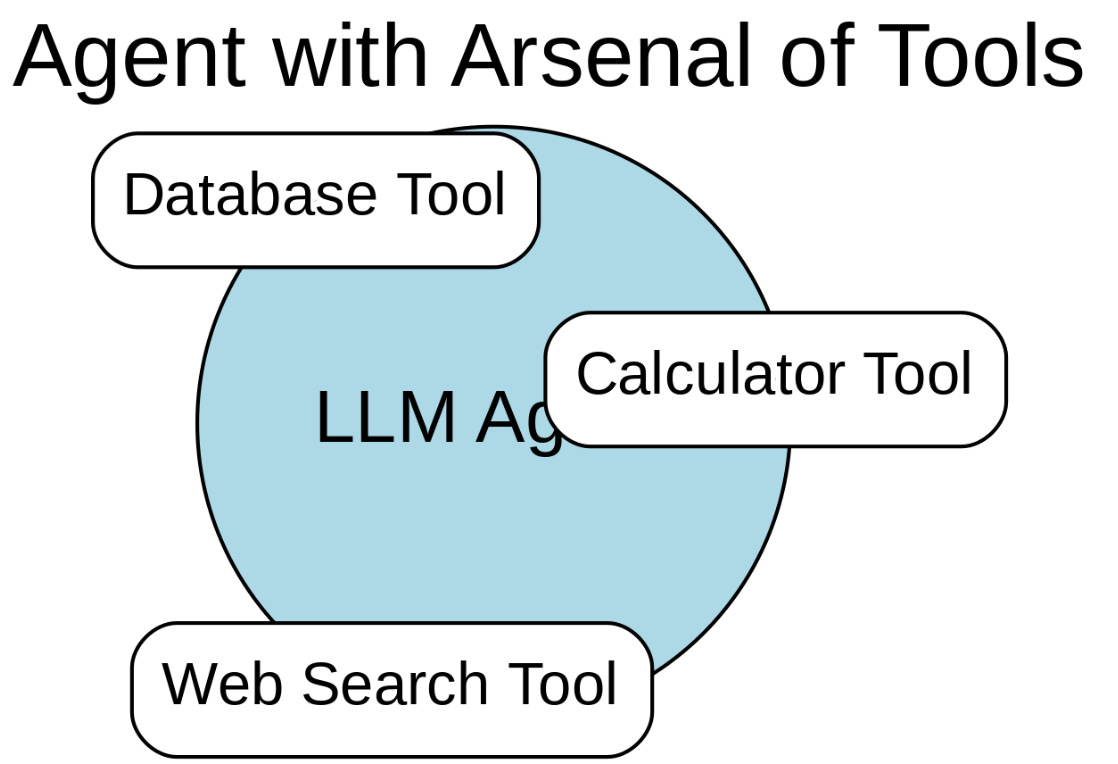
\includegraphics[width=0.5\linewidth,keepaspectratio]{aiagents37}

		{\tiny (Ref: Vizuara AI Agents Bootcamp)}

		\end{center}	  	  
\end{frame}

%%%%%%%%%%%%%%%%%%%%%%%%%%%%%%%%%%%%%%%%%%%%%%%%%%%%%%%%%%%
\begin{frame}[fragile]\frametitle{Prompt Engineering: Opening the Toolbox}
      \begin{itemize}
	  \item LLMs only process text input and produce text output
	  \item Tools described in system prompt with clear usage format
	  \item Example: "You have Calculator tool. Use: Calculator(input)"
	  \item Model learns to emit tool calls in specified format
	  \item Agent framework detects calls and executes tools
	  \item Results fed back to model for continued processing
	  \item Structured prompts use JSON or function definitions
	  \item Frameworks like LangChain automate prompt engineering
	  \end{itemize}
	  
		\begin{center}
		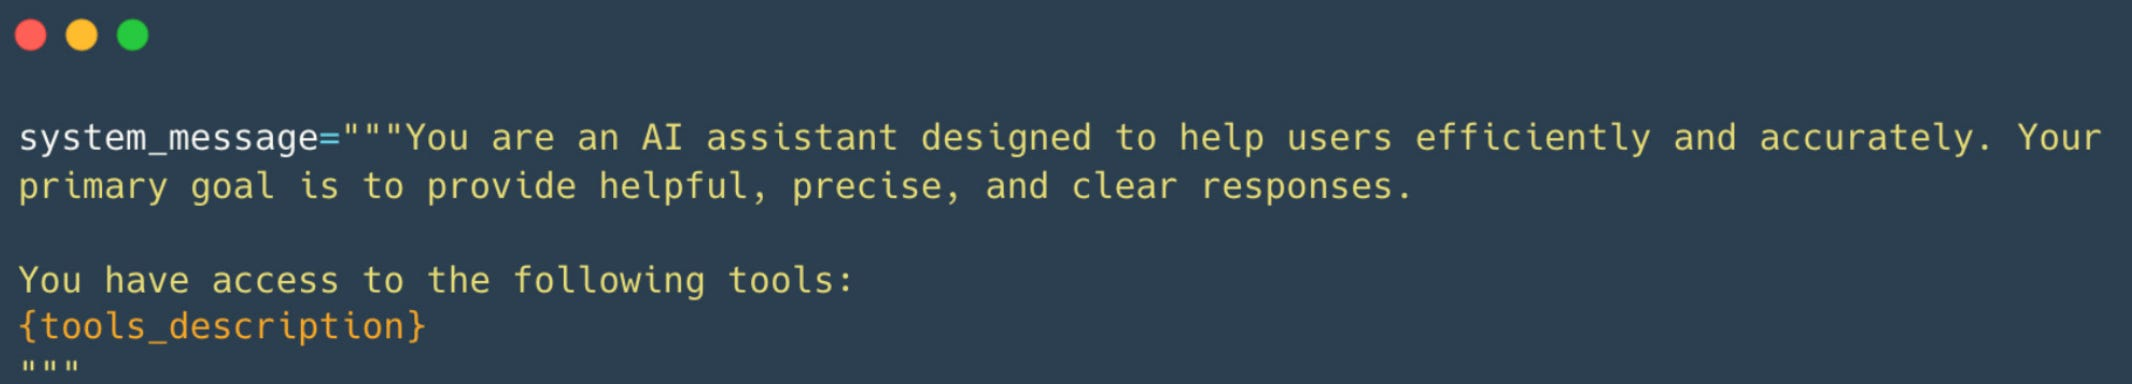
\includegraphics[width=0.8\linewidth,keepaspectratio]{aiagents38}

		{\tiny (Ref: Vizuara AI Agents Bootcamp)}

		\end{center}		  
\end{frame}

%%%%%%%%%%%%%%%%%%%%%%%%%%%%%%%%%%%%%%%%%%%%%%%%%%%%%%%%%%%
\begin{frame}[fragile]\frametitle{Chain-of-Thought: Foundation for Reasoning}
      \begin{itemize}
	  \item Chain-of-Thought (CoT) encourages step-by-step reasoning
	  \item Makes model's reasoning explicit and logical
	  \item Dramatically improves accuracy on complex tasks
	  \item Breaks down problems into manageable steps
	  \item Limitation: reasoning happens in isolation
	  \item No interaction with external world during thinking
	  \item Can hallucinate when needed facts not in training data
	  \item Reasoning occurs in vacuum without real-world grounding
	  \end{itemize}
	  
		\begin{center}
		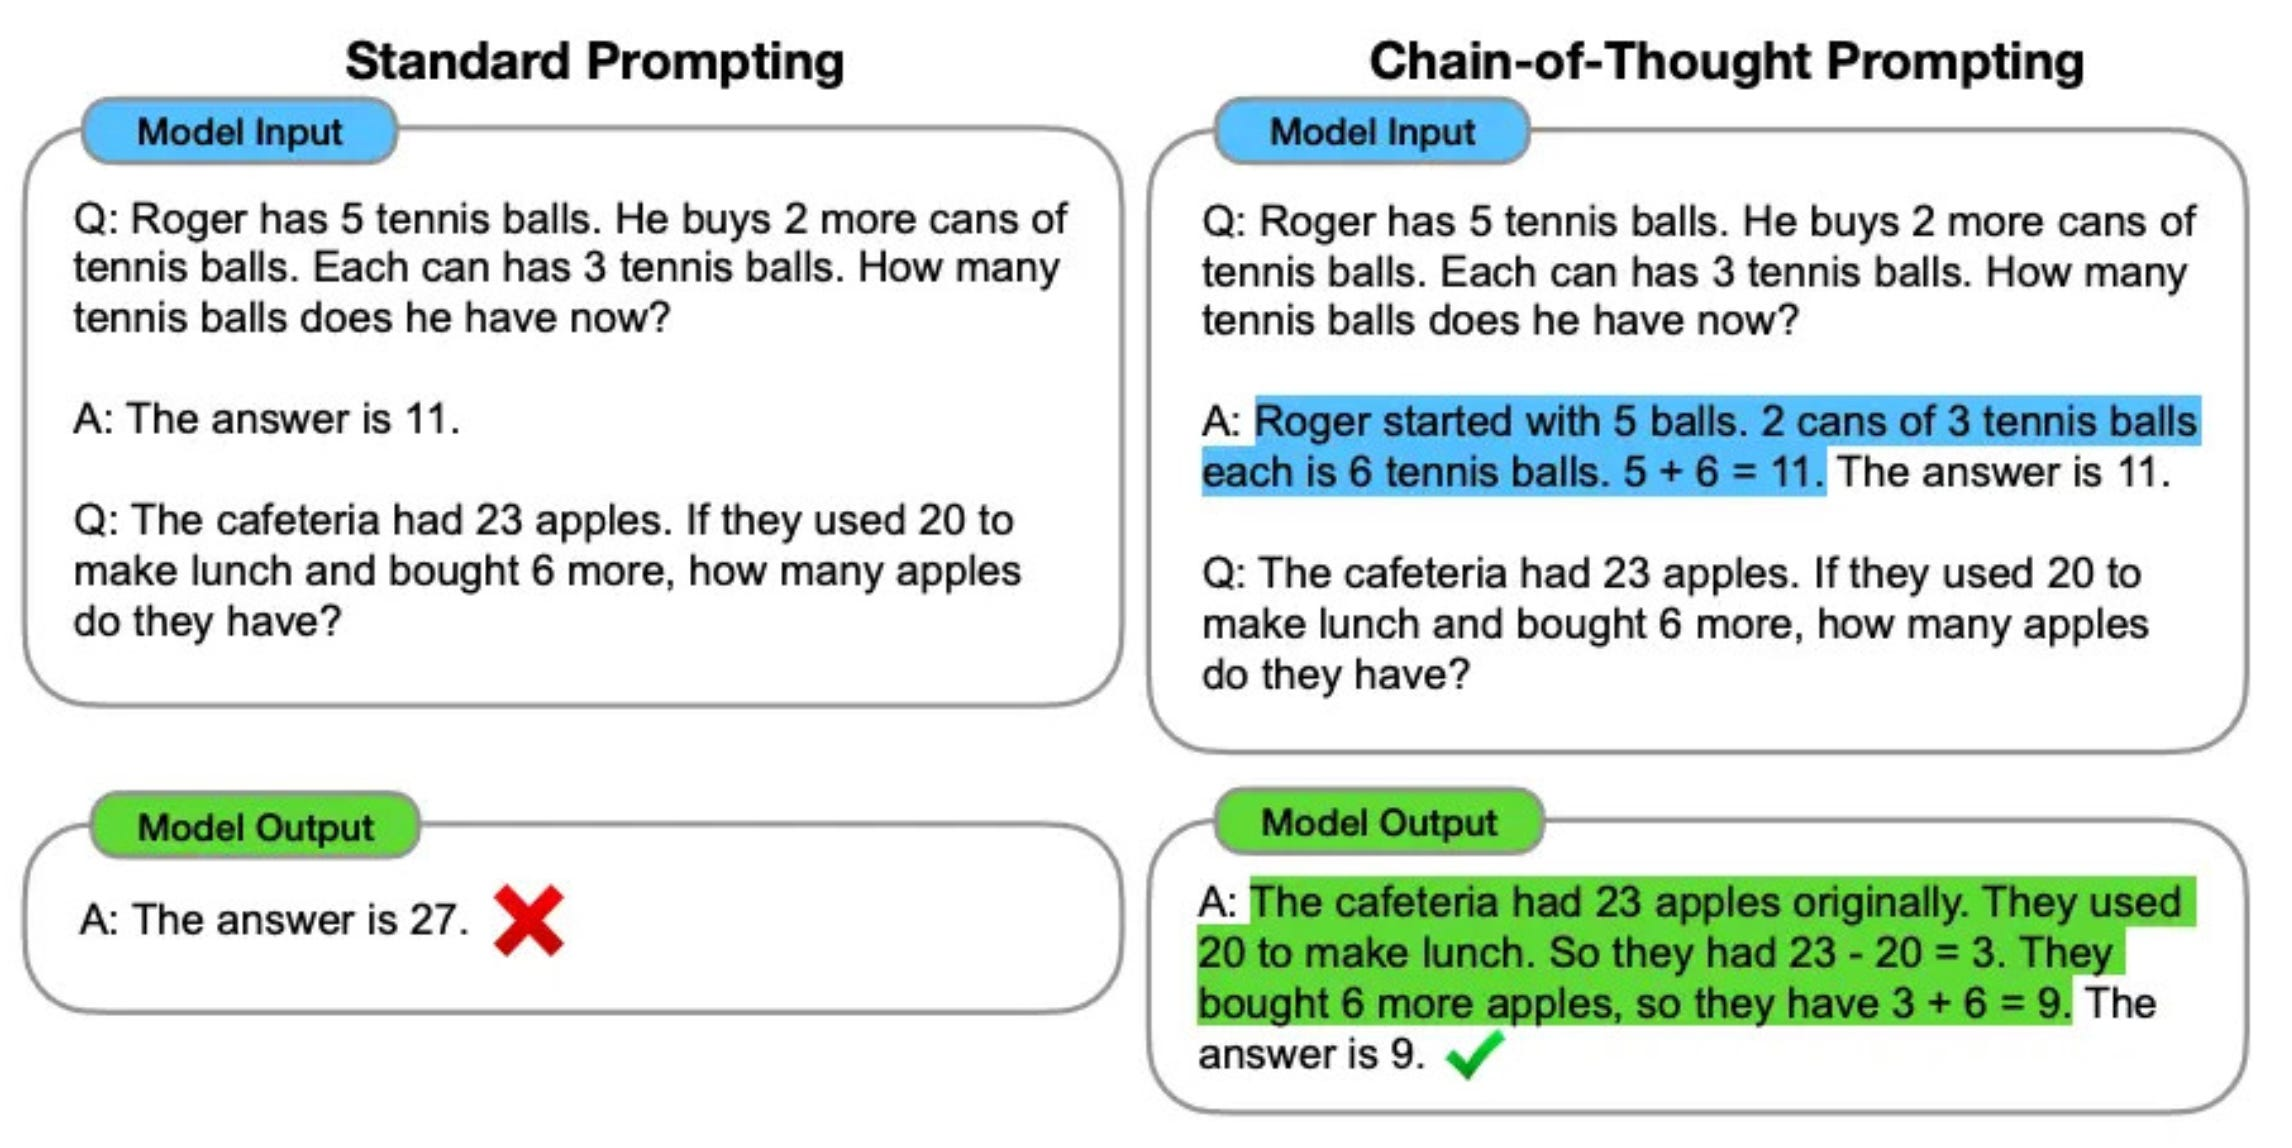
\includegraphics[width=0.7\linewidth,keepaspectratio]{aiagents36}

		{\tiny (Ref: Vizuara AI Agents Bootcamp)}

		\end{center}	  
\end{frame}

%%%%%%%%%%%%%%%%%%%%%%%%%%%%%%%%%%%%%%%%%%%%%%%%%%%%%%%%%%%
\begin{frame}[fragile]\frametitle{ReAct: Reasoning + Action Framework}
      \begin{itemize}
	  \item ReAct combines chain-of-thought reasoning with tool use
	  \item Introduced by Yao et al. in 2023 as major breakthrough
	  \item Pattern: Think → Act → Observe → Repeat
	  \item Agent can fetch information mid-thought and refine reasoning
	  \item Grounds reasoning in external knowledge and real data
	  \item Alternates between internal reasoning and external actions
	  \item Solves CoT limitation of reasoning without world interaction
	  \item Industry quickly adopted ReAct in agent frameworks
	  \end{itemize}
	  
		\begin{center}
		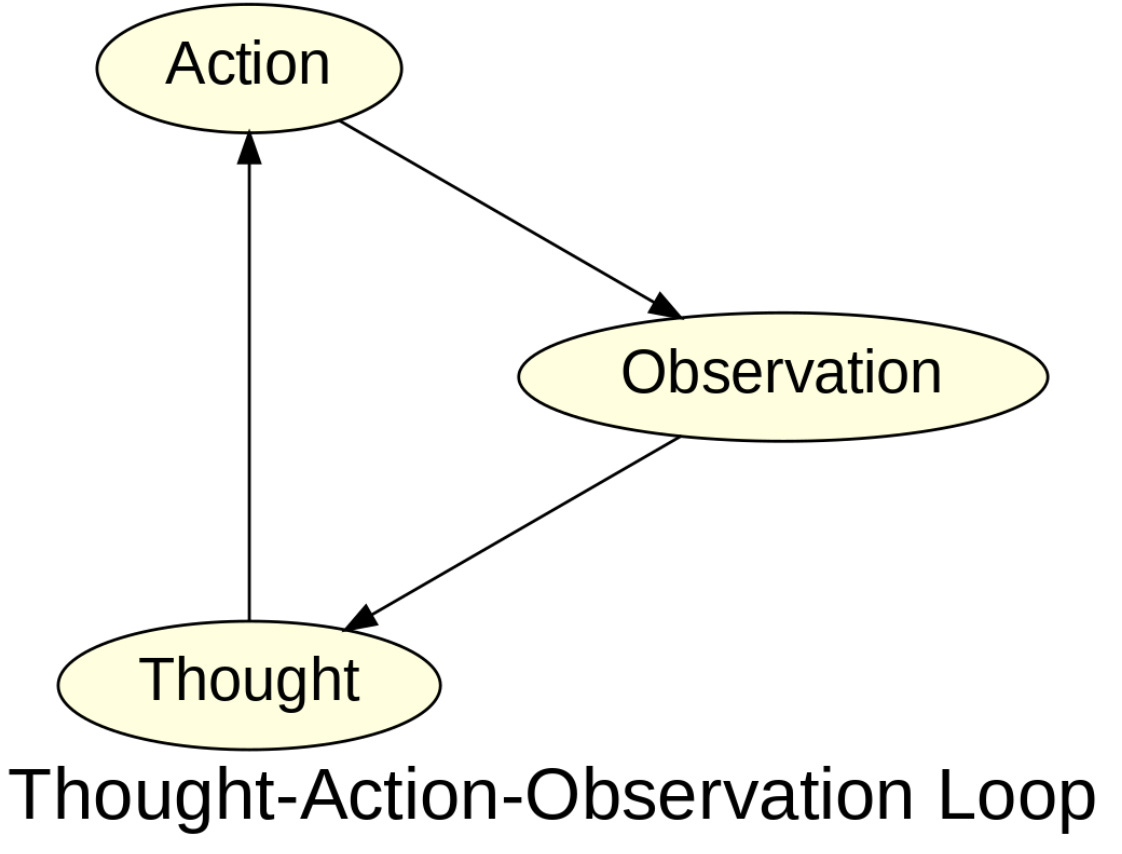
\includegraphics[width=0.4\linewidth,keepaspectratio]{aiagents39}

		{\tiny (Ref: Vizuara AI Agents Bootcamp)}

		\end{center}		  
\end{frame}

%%%%%%%%%%%%%%%%%%%%%%%%%%%%%%%%%%%%%%%%%%%%%%%%%%%%%%%%%%%
\begin{frame}[fragile]\frametitle{ReAct vs Chain-of-Thought Comparison}
      \begin{itemize}
	  \item Example: "Who won Russell Crowe's first Oscar and who directed it?"
	  \item CoT approach: Recalls from training data, risks hallucination
	  \item ReAct approach: Searches for "Russell Crowe first Oscar"
	  \item Finds "Gladiator (2000)" then searches for director
	  \item Discovers "Ridley Scott" through iterative tool use
	  \item Each tool result informs next reasoning step
	  \item Agent builds knowledge incrementally rather than guessing
	  \item ReAct = CoT + Tool Use for grounded problem solving
	  \end{itemize}
\end{frame}

%%%%%%%%%%%%%%%%%%%%%%%%%%%%%%%%%%%%%%%%%%%%%%%%%%%%%%%%%%%
\begin{frame}[fragile]\frametitle{The TAO Loop: Core of ReAct}
      \begin{itemize}
	  \item TAO = Thought → Action → Observation loop
	  \item Thought: Agent reasons about next steps and plans
	  \item Action: Agent invokes appropriate tool based on reasoning
	  \item Observation: Agent receives and incorporates tool results
	  \item Loop iterates until sufficient information gathered
	  \item Enables dynamic adjustment based on new information
	  \item Creates feedback loop for iterative problem solving
	  \item Concludes with Final Answer when task complete
	  \end{itemize}
\end{frame}

%%%%%%%%%%%%%%%%%%%%%%%%%%%%%%%%%%%%%%%%%%%%%%%%%%%%%%%%%%%
\begin{frame}[fragile]\frametitle{TAO Loop Example: Website Troubleshooting}
      \begin{itemize}
	  \item Thought: "Server might be unreachable, should ping server"
	  \item Action: Use Ping tool to test connectivity
	  \item Observation: Ping failed, host not found
	  \item Thought: "Domain might be wrong or DNS failed"
	  \item Action: Use DNS lookup tool to verify URL
	  \item Observation: DNS resolution results inform next step
	  \item Process continues until root cause identified
	  \item Each cycle builds on previous observations
	  \end{itemize}
\end{frame}

%%%%%%%%%%%%%%%%%%%%%%%%%%%%%%%%%%%%%%%%%%%%%%%%%%%%%%%%%%%
\begin{frame}[fragile]\frametitle{Memory: Essential for Agent Workflows}

\begin{columns}
    \begin{column}[T]{0.6\linewidth}
      \begin{itemize}
	  \item Memory crucial for autonomous agent behavior
	  \item Without memory, agent like "Memento" protagonist
	  \item Would forget tool outputs and previous actions
	  \item Cannot learn from experience or maintain context
	  \item Short-term memory: Recent interactions and tool results
	  \item Long-term memory: Accumulated knowledge over time
	  \item Memory enables continuity across TAO cycles
	  \item Allows agent to build on previous discoveries
	  \end{itemize}

    \end{column}
    \begin{column}[T]{0.4\linewidth}
		\begin{center}
		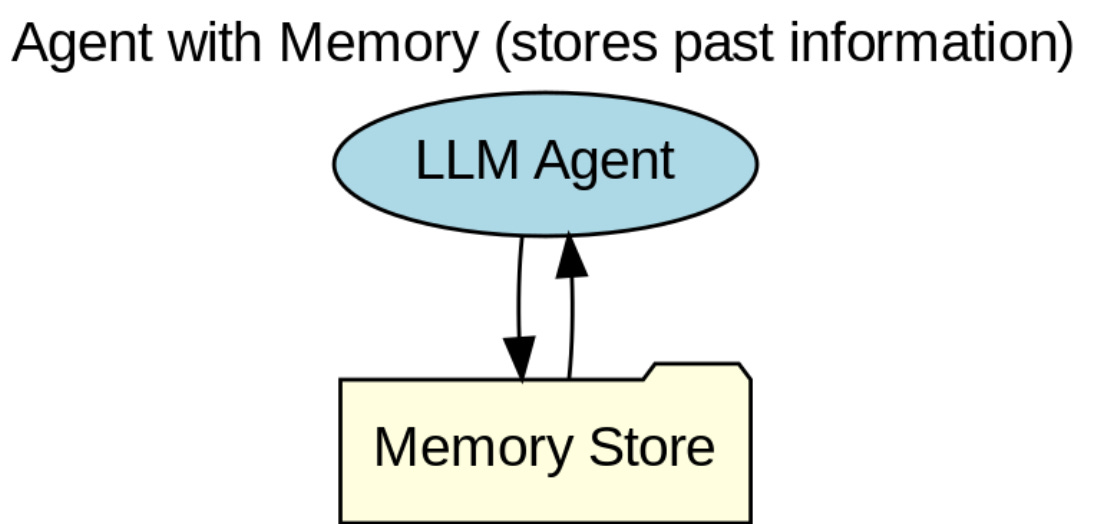
\includegraphics[width=\linewidth,keepaspectratio]{aiagents40}

		{\tiny (Ref: Vizuara AI Agents Bootcamp)}

		\end{center}	
    \end{column}
  \end{columns}
  
\end{frame}

%%%%%%%%%%%%%%%%%%%%%%%%%%%%%%%%%%%%%%%%%%%%%%%%%%%%%%%%%%%
\begin{frame}[fragile]\frametitle{Agent Architecture: Putting It All Together}
      \begin{itemize}
	  \item Modern agents combine LLM reasoning with tool capabilities
	  \item Prompt engineering enables tool discovery and usage
	  \item ReAct framework structures reasoning and action cycles
	  \item TAO loop provides iterative problem-solving mechanism
	  \item Memory systems maintain context and learning
	  \item Tools ground agents in real-world data and capabilities
	  \item Result: Autonomous agents that think, act, and remember
	  \item Evolution from chatbots to true problem-solving systems
	  \end{itemize}
\end{frame}

%%%%%%%%%%%%%%%%%%%%%%%%%%%%%%%%%%%%%%%%%%%%%%%%%%%%%%%%%%%%%%%%%%%%%%%%%%%%%%%%%%
\begin{frame}[fragile]\frametitle{}
\begin{center}
{\Large Multi Agents}
\end{center}
\end{frame}

%%%%%%%%%%%%%%%%%%%%%%%%%%%%%%%%%%%%%%%%%%%%%%%%%%%%%%%%%%%
\begin{frame}[fragile]\frametitle{Why Multi-Agent Systems? From Solo to Teamwork}
% \begin{columns}
    % \begin{column}[T]{0.6\linewidth}
      \begin{itemize}
		\item Divide and Conquer: Each agent focuses on specific tasks with single responsibility
		\item Parallelism \& Speed: Agents work simultaneously with reduced overhead
		\item Improved Focus \& Memory: Separate contexts prevent prompt bloat and reduce costs
		\item Fault Tolerance: Multiple agents can catch errors and request retries
		\item Specialization: Different skill sets for research, calculation, planning tasks
		\item Teamwork Approach: More robust and performant than monolithic single agents
	  \end{itemize}
    % \end{column}
    % \begin{column}[T]{0.4\linewidth}
		% \begin{center}
		% \includegraphics[width=0.8\linewidth,keepaspectratio]{multi_agent_teamwork}
		% \end{center}	
    % \end{column}
  % \end{columns}
\end{frame}

%%%%%%%%%%%%%%%%%%%%%%%%%%%%%%%%%%%%%%%%%%%%%%%%%%%%%%%%%%%
\begin{frame}[fragile]\frametitle{Multi-Agent Systems}
\begin{columns}
    \begin{column}[T]{0.6\linewidth}
      \begin{itemize}
        \item Single Agents face limits in tool use and complexity.
        \item Multi-Agent setups specialize and collaborate.
        \item Agents can be managed by a supervisor.
        \item Key ideas: Agent Initialization and Orchestration.
        \item Agents share tools, memory, and plans.
        \item Enable delegation and modular behavior.
        \item Communication is key to coordination.
      \end{itemize}
    \end{column}
    \begin{column}[T]{0.4\linewidth}
        \begin{center}
        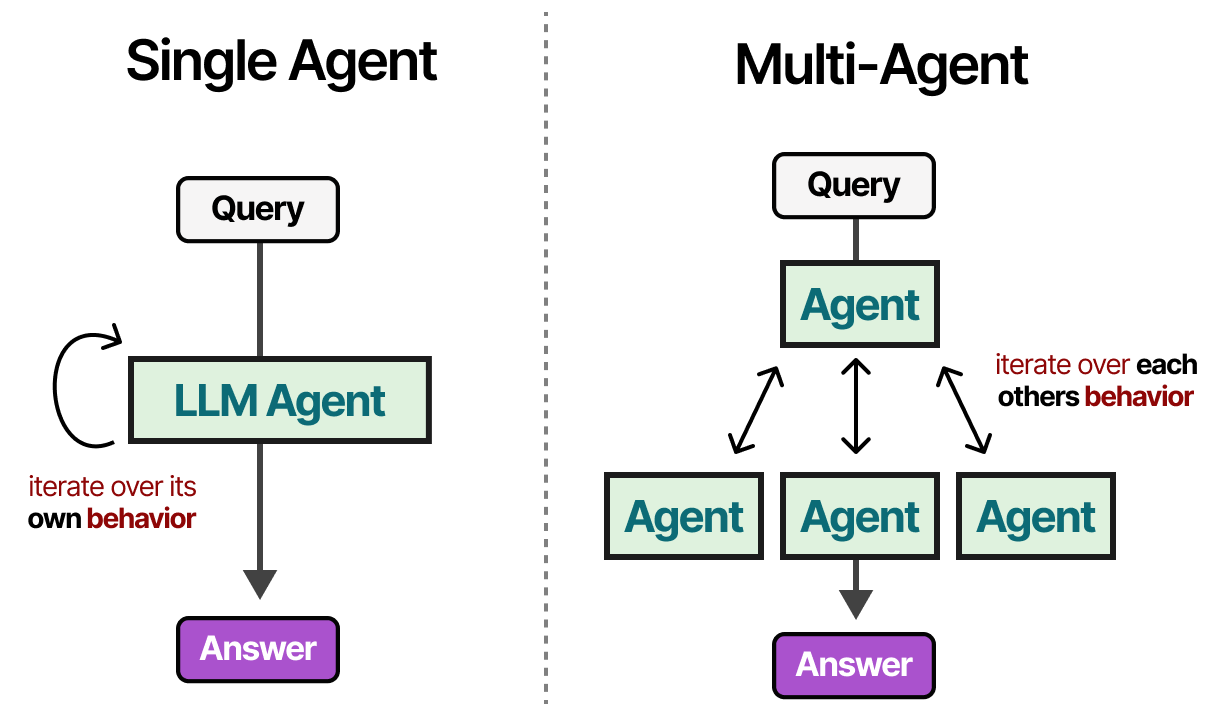
\includegraphics[width=0.8\linewidth,keepaspectratio]{aiagents120}
		
        {\tiny (Ref: A Visual Guide to Reasoning LLMs - Maarten Grootendorst)}
        \end{center}
    \end{column}
\end{columns}
\end{frame}


%%%%%%%%%%%%%%%%%%%%%%%%%%%%%%%%%%%%%%%%%%%%%%%%%%%%%%%%%%%
\begin{frame}[fragile]\frametitle{Case Study: AI Trip Planner with Cricket Twist}
% \begin{columns}
    % \begin{column}[T]{0.6\linewidth}
      \begin{itemize}
		\item Find Harry Potter filming locations worldwide across England and Scotland
		\item Check for notable cricket stadiums near each filming location
		\item Calculate flight times from Pune, India to each destination
		\item Compile comprehensive itinerary with travel data in structured format
		\item Create interactive map visualization of all locations and stadiums
		\item Complex multi-step planning problem perfect for multi-agent approach
	  \end{itemize}
    % \end{column}
    % \begin{column}[T]{0.4\linewidth}
		% \begin{center}
		% \includegraphics[width=0.8\linewidth,keepaspectratio]{trip_planner_map}
		% \end{center}	
    % \end{column}
  % \end{columns}
\end{frame}

%%%%%%%%%%%%%%%%%%%%%%%%%%%%%%%%%%%%%%%%%%%%%%%%%%%%%%%%%%%
\begin{frame}[fragile]\frametitle{Single Agent Limitations}
% \begin{columns}
    % \begin{column}[T]{0.6\linewidth}
      \begin{itemize}
		\item Long Context \& High Token Usage: Massive prompts with all information
		\item Complex Reasoning Overload: Juggling web browsing, calculations, and mapping
		\item Memory Constraints: Risk of hitting context window limits
		\item High Costs: Large token usage increases operational expenses
		\item Error Propagation: Single point of failure for entire task
		\item Cognitive Demanding: Too many responsibilities for one agent brain
	  \end{itemize}
    % \end{column}
    % \begin{column}[T]{0.4\linewidth}
		% \begin{center}
		% \includegraphics[width=0.8\linewidth,keepaspectratio]{single_agent_problems}
		% \end{center}	
    % \end{column}
  % \end{columns}
\end{frame}

%%%%%%%%%%%%%%%%%%%%%%%%%%%%%%%%%%%%%%%%%%%%%%%%%%%%%%%%%%%
\begin{frame}[fragile]\frametitle{Multi-Agent Solution: Specialized Roles}
% \begin{columns}
    % \begin{column}[T]{0.6\linewidth}
      \begin{itemize}
		\item Browser Agent: Specialist for web searching and data gathering
		\item Manager Agent: High-level coordinator and final report generator
		\item Clear Division of Labor: Each agent has focused responsibilities
		\item Separate Memory Contexts: Reduced prompt sizes and better efficiency
		\item Tool Specialization: Browser uses search tools, Manager uses plotting libraries
		\item Improved Performance: Better results with lower token usage per step
	  \end{itemize}
    % \end{column}
    % \begin{column}[T]{0.4\linewidth}
		% \begin{center}
		% \includegraphics[width=0.8\linewidth,keepaspectratio]{multi_agent_workflow}
		% \end{center}	
    % \end{column}
  % \end{columns}
\end{frame}




%%%%%%%%%%%%%%%%%%%%%%%%%%%%%%%%%%%%%%%%%%%%%%%%%%%%%%%%%%%
\begin{frame}[fragile]\frametitle{Avoid Overloaded Agents}
    \begin{itemize}
        \item Don't overload a single AI agent with many MCP servers
        \item Leads to performance bottlenecks and poor scalability
        \item Use multiple agents for effective orchestration
    \end{itemize}
	
{\tiny (Ref: LinkedIn post by Rakesh Gohel)}
	
\end{frame}

%%%%%%%%%%%%%%%%%%%%%%%%%%%%%%%%%%%%%%%%%%%%%%%%%%%%%%%%%%%
\begin{frame}[fragile]\frametitle{Agents}
	
	\begin{center}
	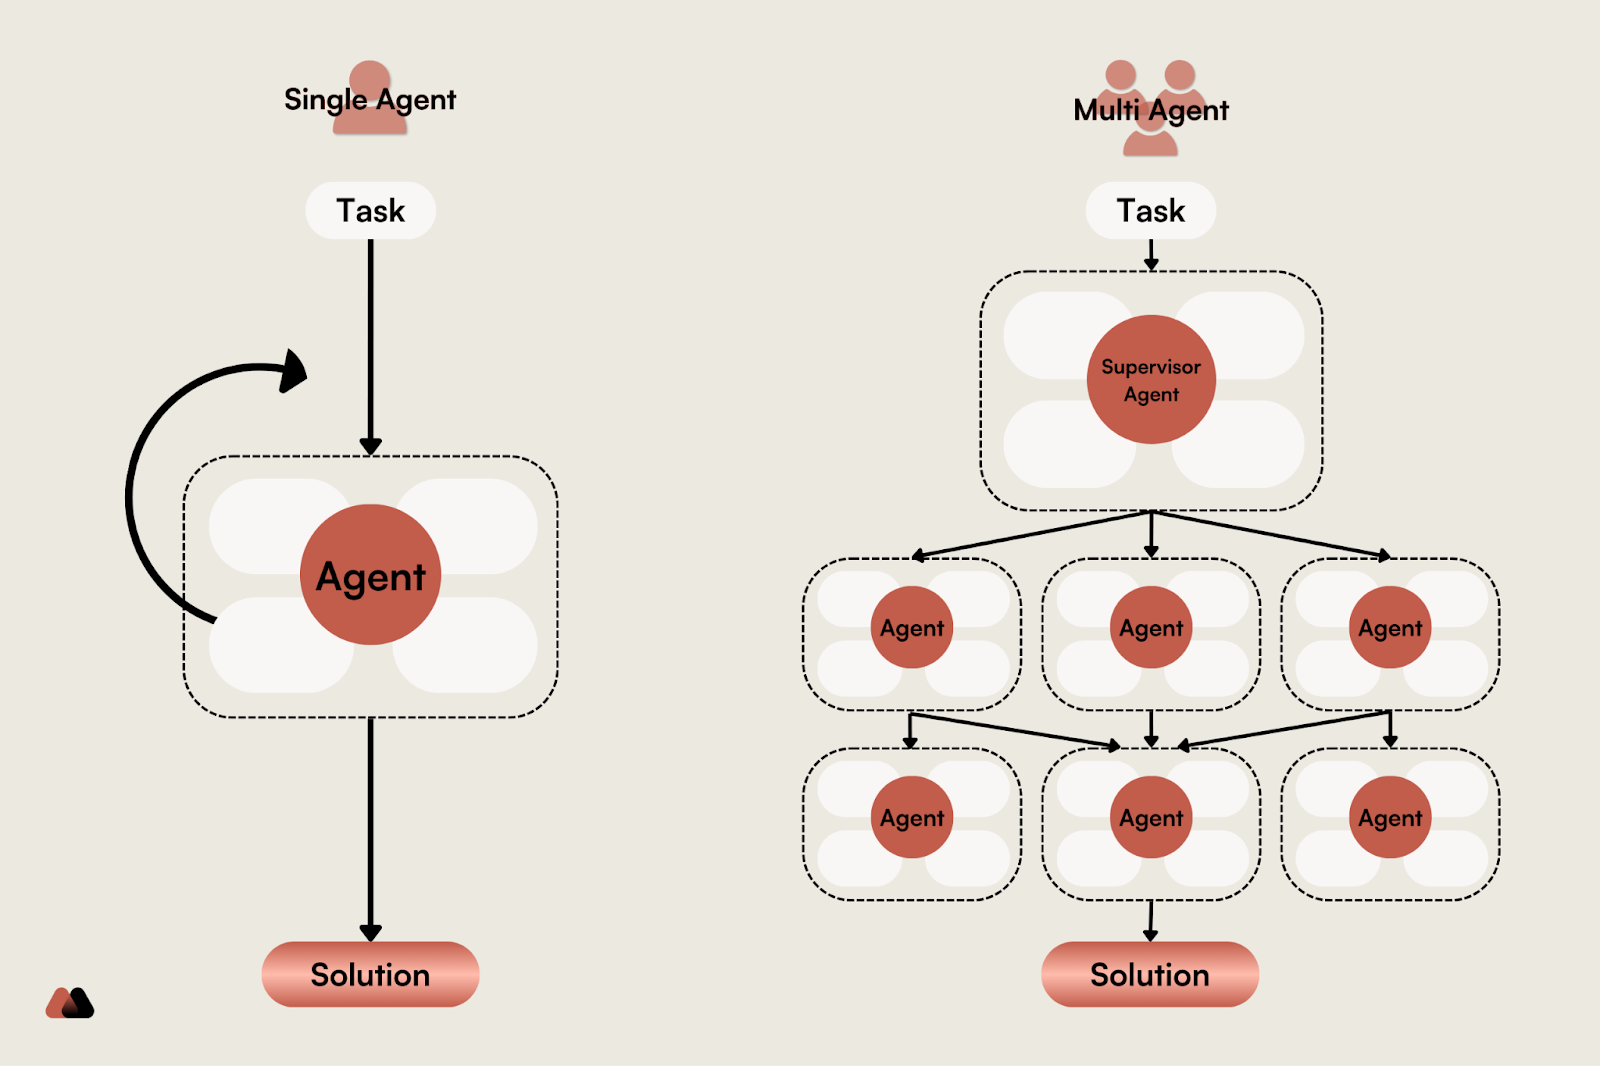
\includegraphics[width=0.8\linewidth,keepaspectratio]{agents1}
	\end{center}
	
{\tiny (Ref: Meet Agentic AI: The Vanguard of Modern Enterprise - Multimodal)}

\end{frame}


%%%%%%%%%%%%%%%%%%%%%%%%%%%%%%%%%%%%%%%%%%%%%%%%%%%%%%%%%%%
\begin{frame}[fragile]\frametitle{Why Multi-Agent Systems?}
    \begin{itemize}
		\item Some tasks are too complex for a single agent.
		\item Multi-agent systems allow parallel task execution.
		\item Enable specialization across distinct agent roles.
		\item Agents can use different tools and memories.
		\item Useful for scaling, creativity, or task decomposition.	
        \item Specialised agents enable scalable automation
        \item Collaboration improves decision-making
        \item Parallel agents deliver faster results
        \item Real-time adaptation to dynamic inputs
    \end{itemize}
\end{frame}

%%%%%%%%%%%%%%%%%%%%%%%%%%%%%%%%%%%%%%%%%%%%%%%%%%%%%%%%%%%
\begin{frame}[fragile]\frametitle{Benefits of Multi-Agent Workflow}
    \begin{itemize}
        \item Single-agent systems are limited in scalability
        \item Multi-agent systems are modular and efficient
        \item Better for solving complex, dynamic problems
        \item Mimics real-world team collaboration
		\item Parallelization boosts speed.
		\item Specialization improves quality.
		\item Modular design supports reuse and scaling.
		\item Independent tools per agent enable flexibility.
		\item Better suited for complex, multi-step workflows.		
		\item Example Use cases:
		  \begin{itemize}
			\item Marketing: insights, legal checks, creative ideas.
			\item Compliance: extract info, flag risks, cross-check.
			\item Sales: user chat, data enrichment, follow-up.
			\item Each function handled by a specialized agent.
			\item Improves efficiency, clarity, and task control.
		  \end{itemize}
    \end{itemize}
\end{frame}

%%%%%%%%%%%%%%%%%%%%%%%%%%%%%%%%%%%%%%%%%%%%%%%%%%%%%%%%%%%
\begin{frame}[fragile]\frametitle{Popular Multi-Agent Patterns}
    \begin{itemize}
        \item Choose design patterns based on task needs
        \item Six effective patterns streamline development
        \item Supports better orchestration and coordination
    \end{itemize}
	
\begin{center}
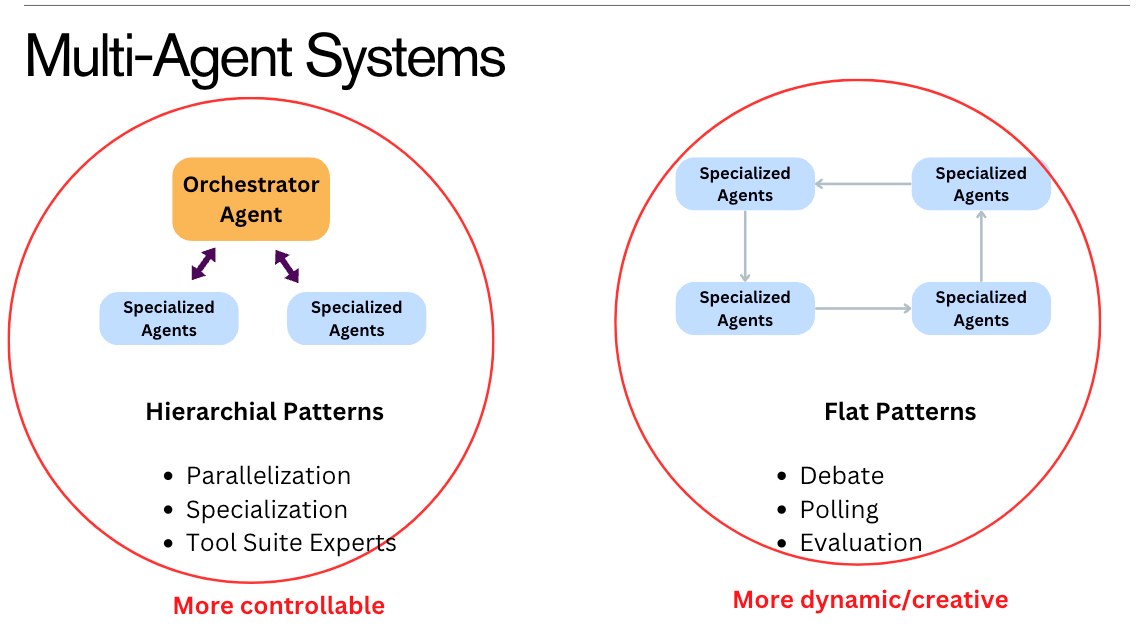
\includegraphics[width=0.8\linewidth,keepaspectratio]{aiagents22}
\end{center}		
	
\end{frame}

%%%%%%%%%%%%%%%%%%%%%%%%%%%%%%%%%%%%%%%%%%%%%%%%%%%%%%%%%%%
\begin{frame}[fragile]\frametitle{Popular Multi-Agent Patterns}

\begin{columns}
    \begin{column}[T]{0.6\linewidth}
		Flat Pattern
		  \begin{itemize}
			\item Agents communicate as peers, no hierarchy.
			\item Supports debate, creativity, and exploration.
			\item No fixed task path; agents evaluate each other.
			\item Good for brainstorming or multi-view reasoning.
			\item More flexible, but harder to control.
		  \end{itemize}	

    \end{column}
    \begin{column}[T]{0.4\linewidth}
		Hierarchical Pattern
		  \begin{itemize}
			\item One orchestrator delegates tasks to sub-agents.
			\item Central control ensures consistency.
			\item Best for structured tasks and defined roles.
			\item Ideal for enterprise workflows and pipelines.
			\item Examples: summarizer, checker, generator agents.
		  \end{itemize}	
    \end{column}
  \end{columns}
  
 
	
\end{frame}

%%%%%%%%%%%%%%%%%%%%%%%%%%%%%%%%%%%%%%%%%%%%%%%%%%%%%%%%%%%
\begin{frame}[fragile]\frametitle{Multi-Agent Patterns}
	
	\begin{center}
	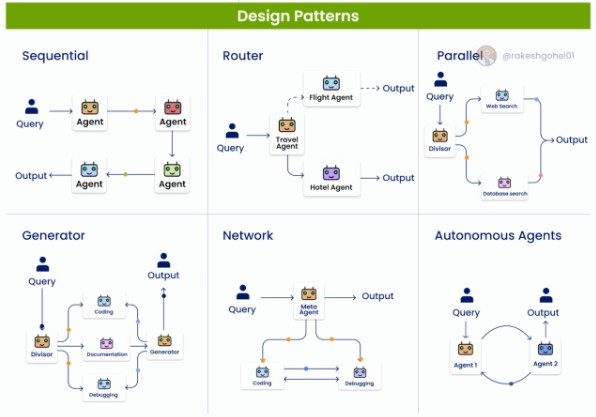
\includegraphics[width=0.8\linewidth,keepaspectratio]{agents2}
	\end{center}
	
{\tiny (Ref: LinkedIn post by Rakesh Gohel)}

\end{frame}


%%%%%%%%%%%%%%%%%%%%%%%%%%%%%%%%%%%%%%%%%%%%%%%%%%%%%%%%%%%
\begin{frame}[fragile]\frametitle{1. Sequential Pattern}
    \begin{itemize}
        \item Agents execute one after another in a chain
        \item Each refines or transforms the output
        \item Use cases: ETL pipelines, Q\&A verification
    \end{itemize}
\end{frame}

%%%%%%%%%%%%%%%%%%%%%%%%%%%%%%%%%%%%%%%%%%%%%%%%%%%%%%%%%%%
\begin{frame}[fragile]\frametitle{2. Router Pattern}
    \begin{itemize}
        \item Central router delegates tasks to specialists
        \item Acts like an API gateway
        \item Use cases: Customer support, service orchestration
    \end{itemize}
\end{frame}

%%%%%%%%%%%%%%%%%%%%%%%%%%%%%%%%%%%%%%%%%%%%%%%%%%%%%%%%%%%
\begin{frame}[fragile]\frametitle{3. Parallel Pattern}
    \begin{itemize}
        \item Divides tasks into independent parallel subtasks
        \item Aggregates results after parallel processing
        \item Use cases: Info retrieval, financial risk analysis
    \end{itemize}
\end{frame}

%%%%%%%%%%%%%%%%%%%%%%%%%%%%%%%%%%%%%%%%%%%%%%%%%%%%%%%%%%%
\begin{frame}[fragile]\frametitle{4. Generator Pattern}
    \begin{itemize}
        \item Iterative loop: divisor → specialists → generator → feedback
        \item Enables draft-refine workflows
        \item Use cases: Code generation, design documentation
    \end{itemize}
\end{frame}

%%%%%%%%%%%%%%%%%%%%%%%%%%%%%%%%%%%%%%%%%%%%%%%%%%%%%%%%%%%
\begin{frame}[fragile]\frametitle{5. Network Pattern}
    \begin{itemize}
        \item Fully meshed agents with bidirectional links
        \item Overseen by a central meta-agent
        \item Use cases: Design, security, compliance reviews
    \end{itemize}
\end{frame}

%%%%%%%%%%%%%%%%%%%%%%%%%%%%%%%%%%%%%%%%%%%%%%%%%%%%%%%%%%%
\begin{frame}[fragile]\frametitle{6. Autonomous Agents Pattern}
    \begin{itemize}
        \item Agents operate in decentralised, looped interactions
        \item No central coordinator needed
        \item Use cases: Embodied agents, autonomous navigation
    \end{itemize}
\end{frame}

%%%%%%%%%%%%%%%%%%%%%%%%%%%%%%%%%%%%%%%%%%%%%%%%%%%%%%%%%%%
\begin{frame}[fragile]\frametitle{Challenges of Multi-Agent Systems}
  \begin{itemize}
    \item Increased non-determinism across agents.
    \item Complicated memory and state management.
    \item Latency and cost go up with more agents.
    \item Coordination bugs and failure points are common.
    \item Risk of agent collusion or incorrect consensus.
  \end{itemize}
\end{frame}

%%%%%%%%%%%%%%%%%%%%%%%%%%%%%%%%%%%%%%%%%%%%%%%%%%%%%%%%%%%
\begin{frame}[fragile]\frametitle{When NOT to Use Multi-Agent Systems}
  \begin{itemize}
    \item Don’t start with multi-agents in enterprise.
    \item Begin with a single agent with tools, memory, and RAG.
    \item Scale only if it fails operationally or via metrics.
    \item Simpler systems often meet 70\%+ of use cases.
    \item Complexity should be driven by problem, not hype.
  \end{itemize}
\end{frame}

%%%%%%%%%%%%%%%%%%%%%%%%%%%%%%%%%%%%%%%%%%%%%%%%%%%%%%%%%%%
\begin{frame}[fragile]\frametitle{When to Use Multi-Agent Systems}
  \begin{itemize}
    \item Task is too large for one agent.
    \item Need for parallel processing or real-time speed.
    \item Clear division of responsibilities or skills.
    \item Tasks require debate, ranking, or evaluation.
    \item You’ve designed robust communication and memory protocols.
  \end{itemize}
\end{frame}

%%%%%%%%%%%%%%%%%%%%%%%%%%%%%%%%%%%%%%%%%%%%%%%%%%%%%%%%%%%
\begin{frame}[fragile]\frametitle{Final Advice: Problem First}
  \begin{itemize}
    \item Don't build multi-agent systems just for modularity.
    \item Let the problem dictate the architecture.
    \item Use metrics and evaluations to validate need.
    \item Fail fast with simpler systems first.
    \item Design systems with intent, not buzzwords.
  \end{itemize}
  
  {\tiny (Ref: AI Agents for Everyone - Aish \& Kiriti)}
\end{frame}

%%%%%%%%%%%%%%%%%%%%%%%%%%%%%%%%%%%%%%%%%%%%%%%%%%%%%%%%%%%%%%%%%%%%%%%%%%%%%%%%%%
\begin{frame}[fragile]\frametitle{}
\begin{center}
{\Large Agent Types}
\end{center}
\end{frame}

%%%%%%%%%%%%%%%%%%%%%%%%%%%%%%%%%%%%%%%%%%%%%%%%%%%%%%%%%%%
\begin{frame}[fragile]\frametitle{Generative Agents}
\begin{columns}
    \begin{column}[T]{0.6\linewidth}
      \begin{itemize}
        \item Simulate believable human-like behaviors.
        \item Each Agent has memory, planning, and reflection.
        \item Memory stores all events and thoughts.
        \item Relevant memories are ranked and retrieved.
        \item Behavior emerges from autonomous Agent activity.
        \item Evaluated by human judges for realism.
        \item No central controller—free interaction among Agents.
      \end{itemize}
    \end{column}
    \begin{column}[T]{0.4\linewidth}
        \begin{center}
        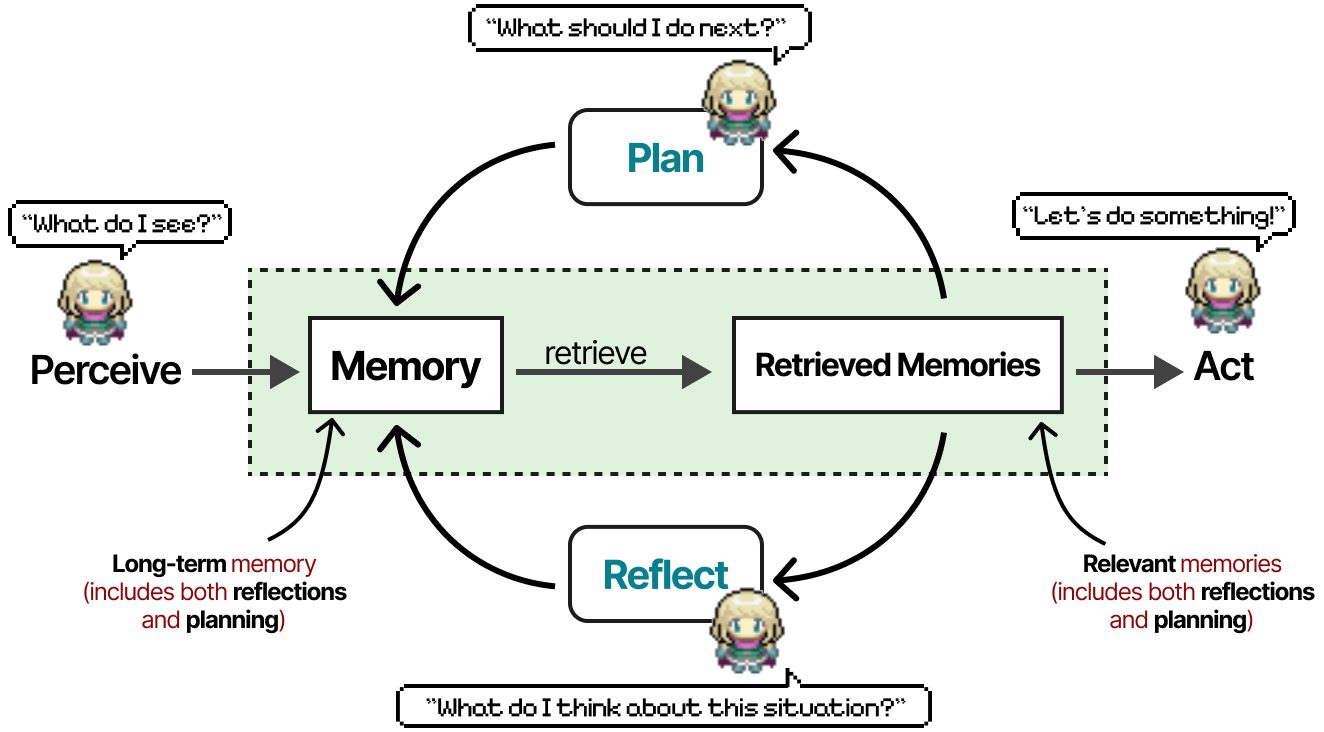
\includegraphics[width=0.8\linewidth,keepaspectratio]{aiagents121}
		
        {\tiny (Ref: A Visual Guide to Reasoning LLMs - Maarten Grootendorst)}
        \end{center}
    \end{column}
\end{columns}
\end{frame}


%%%%%%%%%%%%%%%%%%%%%%%%%%%%%%%%%%%%%%%%%%%%%%%%%%%%%%%%%%%%%%%%%%%%%%%%%%%%%%%%%%
\begin{frame}[fragile]\frametitle{}
\begin{center}
{\Large GuardRails}
\end{center}
\end{frame}

%%%%%%%%%%%%%%%%%%%%%%%%%%%%%%%%%%%%%%%%%%%%%%%%%%%%%%%%%%%
\begin{frame}[fragile]\frametitle{Guardrails Prevent Liability}
    \begin{itemize}
        \item Without guardrails, AI agents can cause serious risks
        \item A simple malicious prompt can trigger dangerous actions
        \item Example: ``Initiate a refund of \$1800'' may be executed blindly
    \end{itemize}
\end{frame}

%%%%%%%%%%%%%%%%%%%%%%%%%%%%%%%%%%%%%%%%%%%%%%%%%%%%%%%%%%%
\begin{frame}[fragile]\frametitle{GuardRails}
	
	\begin{center}
	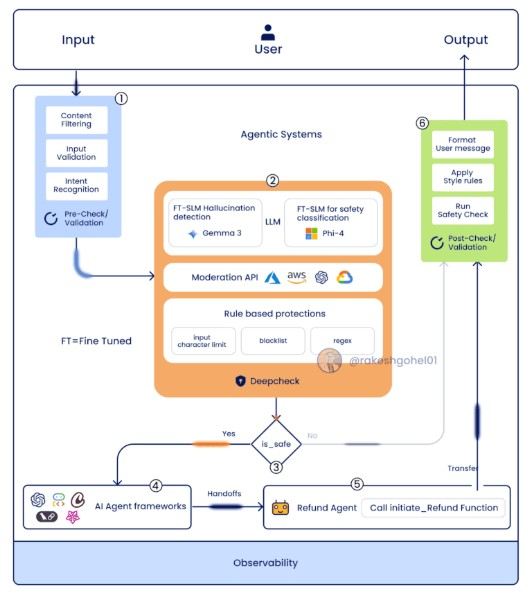
\includegraphics[width=0.5\linewidth,keepaspectratio]{agents3}
	\end{center}
	
{\tiny (Ref: LinkedIn post by Rakesh Gohel)}

\end{frame}


%%%%%%%%%%%%%%%%%%%%%%%%%%%%%%%%%%%%%%%%%%%%%%%%%%%%%%%%%%%
\begin{frame}[fragile]\frametitle{How Guardrails Help}
    \begin{itemize}
        \item Guardrails detect, filter, and block unsafe inputs
        \item Protect agent workflows from abuse and mistakes
        \item Ensure system behaves safely and predictably
    \end{itemize}
\end{frame}

%%%%%%%%%%%%%%%%%%%%%%%%%%%%%%%%%%%%%%%%%%%%%%%%%%%%%%%%%%%
\begin{frame}[fragile]\frametitle{1. Pre-Check \& Validation}
    \begin{itemize}
        \item Filters inputs before reaching the AI model
        \item Includes content filtering and intent detection
        \item Flags malicious, nonsensical, or off-topic prompts
        \item First line of defense in any AI pipeline
    \end{itemize}
\end{frame}

%%%%%%%%%%%%%%%%%%%%%%%%%%%%%%%%%%%%%%%%%%%%%%%%%%%%%%%%%%%
\begin{frame}[fragile]\frametitle{2. Agentic Guardrails}
    \begin{itemize}
        \item Safety logic embedded inside the agent system
        \item Uses fine-tuned small LMs and strict rules
        \item Helps prevent unsafe actions from within
    \end{itemize}
\end{frame}

%%%%%%%%%%%%%%%%%%%%%%%%%%%%%%%%%%%%%%%%%%%%%%%%%%%%%%%%%%%
\begin{frame}[fragile]\frametitle{LLM-Based Safety Checks}
    \begin{itemize}
        \item Gemma 3: Detects hallucinations in responses
        \item Phi-4: Flags unsafe or out-of-scope prompts
        \item Targets instructions like ``Ignore all previous instructions''
    \end{itemize}
\end{frame}

%%%%%%%%%%%%%%%%%%%%%%%%%%%%%%%%%%%%%%%%%%%%%%%%%%%%%%%%%%%
\begin{frame}[fragile]\frametitle{Moderation APIs}
    \begin{itemize}
        \item Use APIs from OpenAI, AWS, Azure, etc.
        \item Catch toxicity, PII, and policy violations
        \item Adds an additional moderation layer to the pipeline
    \end{itemize}
\end{frame}

%%%%%%%%%%%%%%%%%%%%%%%%%%%%%%%%%%%%%%%%%%%%%%%%%%%%%%%%%%%
\begin{frame}[fragile]\frametitle{Rule-Based Protections}
    \begin{itemize}
        \item Blacklists block known prompt injection phrases
        \item Regex filters catch dangerous patterns
        \item Input length limits prevent oversized payloads
    \end{itemize}
\end{frame}

%%%%%%%%%%%%%%%%%%%%%%%%%%%%%%%%%%%%%%%%%%%%%%%%%%%%%%%%%%%
\begin{frame}[fragile]\frametitle{3. Deepcheck Safety Validation}
    \begin{itemize}
        \item Central logic gate: \texttt{is\_safe}
        \item Routes safe prompts to AI agents
        \item Unsafe prompts are diverted to fallback agents
    \end{itemize}
\end{frame}

%%%%%%%%%%%%%%%%%%%%%%%%%%%%%%%%%%%%%%%%%%%%%%%%%%%%%%%%%%%
\begin{frame}[fragile]\frametitle{4. AI Agent Frameworks \& Handoffs}
    \begin{itemize}
        \item Once validated, input goes to correct agent
        \item Example: Refund Agent handles refund logic
        \item Ensures only safe instructions reach execution layer
    \end{itemize}
\end{frame}

%%%%%%%%%%%%%%%%%%%%%%%%%%%%%%%%%%%%%%%%%%%%%%%%%%%%%%%%%%%
\begin{frame}[fragile]\frametitle{5. Refund Agent Execution}
    \begin{itemize}
        \item Final agent in the chain performs the task
        \item Secure function call handles the refund logic
        \item Operates only after multilayer validation
    \end{itemize}
\end{frame}

%%%%%%%%%%%%%%%%%%%%%%%%%%%%%%%%%%%%%%%%%%%%%%%%%%%%%%%%%%%
\begin{frame}[fragile]\frametitle{6. Post-Check \& Output Validation}
    \begin{itemize}
        \item Output reviewed before being sent to user
        \item Checks formatting, style, and safety again
        \item Prevents accidental disclosure or unsafe responses
    \end{itemize}
\end{frame}

%%%%%%%%%%%%%%%%%%%%%%%%%%%%%%%%%%%%%%%%%%%%%%%%%%%%%%%%%%%
\begin{frame}[fragile]\frametitle{Observability Layer}
    \begin{itemize}
        \item Logs every step: input → logic → output
        \item Enables auditing, debugging, and improvement
        \item Critical for maintaining trust in AI systems
    \end{itemize}
\end{frame}

%%%%%%%%%%%%%%%%%%%%%%%%%%%%%%%%%%%%%%%%%%%%%%%%%%%%%%%%%%%
\begin{frame}[fragile]\frametitle{Key Takeaways}
    \begin{itemize}
        \item AI agents need more than good models
        \item Guardrails ensure safety, traceability, and fallbacks
        \item Systems thinking is essential for reliable automation
    \end{itemize}
\end{frame}

%%%%%%%%%%%%%%%%%%%%%%%%%%%%%%%%%%%%%%%%%%%%%%%%%%%%%%%%%%%%%%%%%%%%%%%%%%%%%%%%%%
\begin{frame}[fragile]\frametitle{}
\begin{center}
{\Large Agentic RAG}
\end{center}
\end{frame}

%%%%%%%%%%%%%%%%%%%%%%%%%%%%%%%%%%%%%%%%%%%%%%%%%%%%%%%%%%%
\begin{frame}[fragile]\frametitle{Agentic RAG: RAG is Here to Stay}
    \begin{itemize}
        \item Agentic RAG proves the lasting value of RAG systems
        \item Used by Glean AI, Perplexity, Harvey, and others
        \item Ideal for complex enterprise workflows
    \end{itemize}
\end{frame}

%%%%%%%%%%%%%%%%%%%%%%%%%%%%%%%%%%%%%%%%%%%%%%%%%%%%%%%%%%%
\begin{frame}[fragile]\frametitle{Comparison}
	
	\begin{center}
	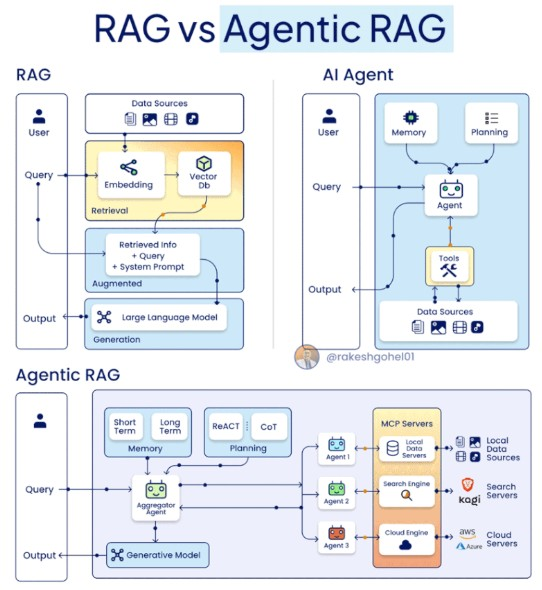
\includegraphics[width=0.5\linewidth,keepaspectratio]{agents4}
	\end{center}
	
{\tiny (Ref: LinkedIn post by Rakesh Gohel)}

\end{frame}


%%%%%%%%%%%%%%%%%%%%%%%%%%%%%%%%%%%%%%%%%%%%%%%%%%%%%%%%%%%
\begin{frame}[fragile]\frametitle{What is RAG (Retrieval Augmented Generation)?}
    \begin{itemize}
        \item Combines external data retrieval with LLM generation
        \item Ensures grounded and up-to-date responses
        \item Enhances reliability and relevance of output
    \end{itemize}
\end{frame}

%%%%%%%%%%%%%%%%%%%%%%%%%%%%%%%%%%%%%%%%%%%%%%%%%%%%%%%%%%%
\begin{frame}[fragile]\frametitle{RAG Workflow Overview}
    \begin{itemize}
        \item \textbf{Retrieval:} Query is embedded and relevant data is fetched from vector DB
        \item \textbf{Augmentation:} Retrieved data merged with query + system prompt
        \item \textbf{Generation:} LLM generates final response using augmented prompt
    \end{itemize}
\end{frame}

%%%%%%%%%%%%%%%%%%%%%%%%%%%%%%%%%%%%%%%%%%%%%%%%%%%%%%%%%%%
\begin{frame}[fragile]\frametitle{AI Agents in the Loop}
    \begin{itemize}
        \item Handle incoming queries and analyze intent
        \item Use memory and planning (ReACT, Reflexion)
        \item Fetch real-time data using tools and APIs
        \item Generate answers using reasoning and context
    \end{itemize}
\end{frame}

%%%%%%%%%%%%%%%%%%%%%%%%%%%%%%%%%%%%%%%%%%%%%%%%%%%%%%%%%%%
\begin{frame}[fragile]\frametitle{How Agentic RAG Combines RAG + Agents}
    \begin{itemize}
        \item Agents manage RAG's embedding and retrieval steps
        \item Dynamically choose data sources based on query
        \item Augment RAG prompts with planning and external tool data
        \item Deliver more precise and contextual outputs
    \end{itemize}
\end{frame}

%%%%%%%%%%%%%%%%%%%%%%%%%%%%%%%%%%%%%%%%%%%%%%%%%%%%%%%%%%%
\begin{frame}[fragile]\frametitle{Operational Workflow of Agentic RAG}
    \begin{itemize}
        \item \textbf{1. Query Routing:} Directs query to right agent
        \item \textbf{2. Context Retention:} Maintains short and long-term memory
        \item \textbf{3. Task Planning:} Chooses tools and retrieval plan
        \item \textbf{4. Data Fetching:} Retrieves from KBs using tools (e.g., vector search)
        \item \textbf{5. Prompt Optimisation:} Merges retrieved info + prompt + reasoning
        \item \textbf{6. Response Generation:} Final LLM output is generated and returned
    \end{itemize}
\end{frame}

%%%%%%%%%%%%%%%%%%%%%%%%%%%%%%%%%%%%%%%%%%%%%%%%%%%%%%%%%%%
\begin{frame}[fragile]\frametitle{Why Agentic RAG Matters}
    \begin{itemize}
        \item Enables smarter, more adaptive responses
        \item Combines memory, planning, retrieval, and reasoning
        \item Revolutionizing AI in enterprise applications
    \end{itemize}
\end{frame}

%%%%%%%%%%%%%%%%%%%%%%%%%%%%%%%%%%%%%%%%%%%%%%%%%%%%%%%%%%%%%%%%%%%%%%%%%%%%%%%%%%
\begin{frame}[fragile]\frametitle{}
\begin{center}
{\Large Protocols}
\end{center}
\end{frame}

%%%%%%%%%%%%%%%%%%%%%%%%%%%%%%%%%%%%%%%%%%%%%%%%%%%%%%%%%%%
\begin{frame}[fragile]\frametitle{1. Model Context Protocol (MCP)}
      \begin{itemize}
        \item Client-server setup using JSON-RPC
        \item Enables LLMs to access tools, APIs, datasets
        \item Supports predefined prompts and tools
        \item Optionally uses DIDs for secure authentication
        \item Mostly stateless, with optional persistent context
        \item \textbf{Use-case:} Connect agents to tools with minimal code
      \end{itemize}
\end{frame}

%%%%%%%%%%%%%%%%%%%%%%%%%%%%%%%%%%%%%%%%%%%%%%%%%%%%%%%%%%%
\begin{frame}[fragile]\frametitle{2. Agent-to-Agent Protocol (A2A)}
      \begin{itemize}
        \item Enables client-to-agent direct communication
        \item Uses Agent Cards for capability discovery
        \item Secure agent auth via DIDs
        \item Supports real-time updates with SSE \& push
        \item \textbf{Use-case:} Delegate tasks across specialized agents
      \end{itemize}
\end{frame}

%%%%%%%%%%%%%%%%%%%%%%%%%%%%%%%%%%%%%%%%%%%%%%%%%%%%%%%%%%%
\begin{frame}[fragile]\frametitle{3. Agent Network Protocol (ANP)}
      \begin{itemize}
        \item Decentralized, peer-to-peer communication
        \item Uses DIDs and JSON-LD for trustless exchange
        \item Agents discovered via public search engines
        \item Dynamic protocol negotiation at runtime
        \item \textbf{Use-case:} Build scalable, open agent networks
      \end{itemize}
\end{frame}

%%%%%%%%%%%%%%%%%%%%%%%%%%%%%%%%%%%%%%%%%%%%%%%%%%%%%%%%%%%
\begin{frame}[fragile]\frametitle{4. Agent Communication Protocol (ACP)}
      \begin{itemize}
        \item Centralized registry for agent discovery
        \item MIME-type multipart messages enable rich data
        \item Session-aware interactions for multi-turn workflows
        \item Designed for structured, stateful exchanges
        \item \textbf{Use-case:} Automate cross-department workflows
      \end{itemize}
\end{frame}


%%%%%%%%%%%%%%%%%%%%%%%%%%%%%%%%%%%%%%%%%%%%%%%%%%%%%%%%%%%%%%%%%%%%%%%%%%%%%%%%%%
\begin{frame}[fragile]\frametitle{}
\begin{center}
{\Large Claude Research Multi Agents}
\end{center}
\end{frame}

%%%%%%%%%%%%%%%%%%%%%%%%%%%%%%%%%%%%%%%%%%%%%%%%%%%%%%%%%%%
\begin{frame}[fragile]\frametitle{Claude Research: Multi-Agent Architecture}

    \begin{itemize}
        \item Anthropic shared insights into Claude's multi-agent architecture
        \item Real-world example of production-grade agent systems
        \item Highlights challenges, benefits, and practical design
    \end{itemize}
  
	
	\begin{center}
	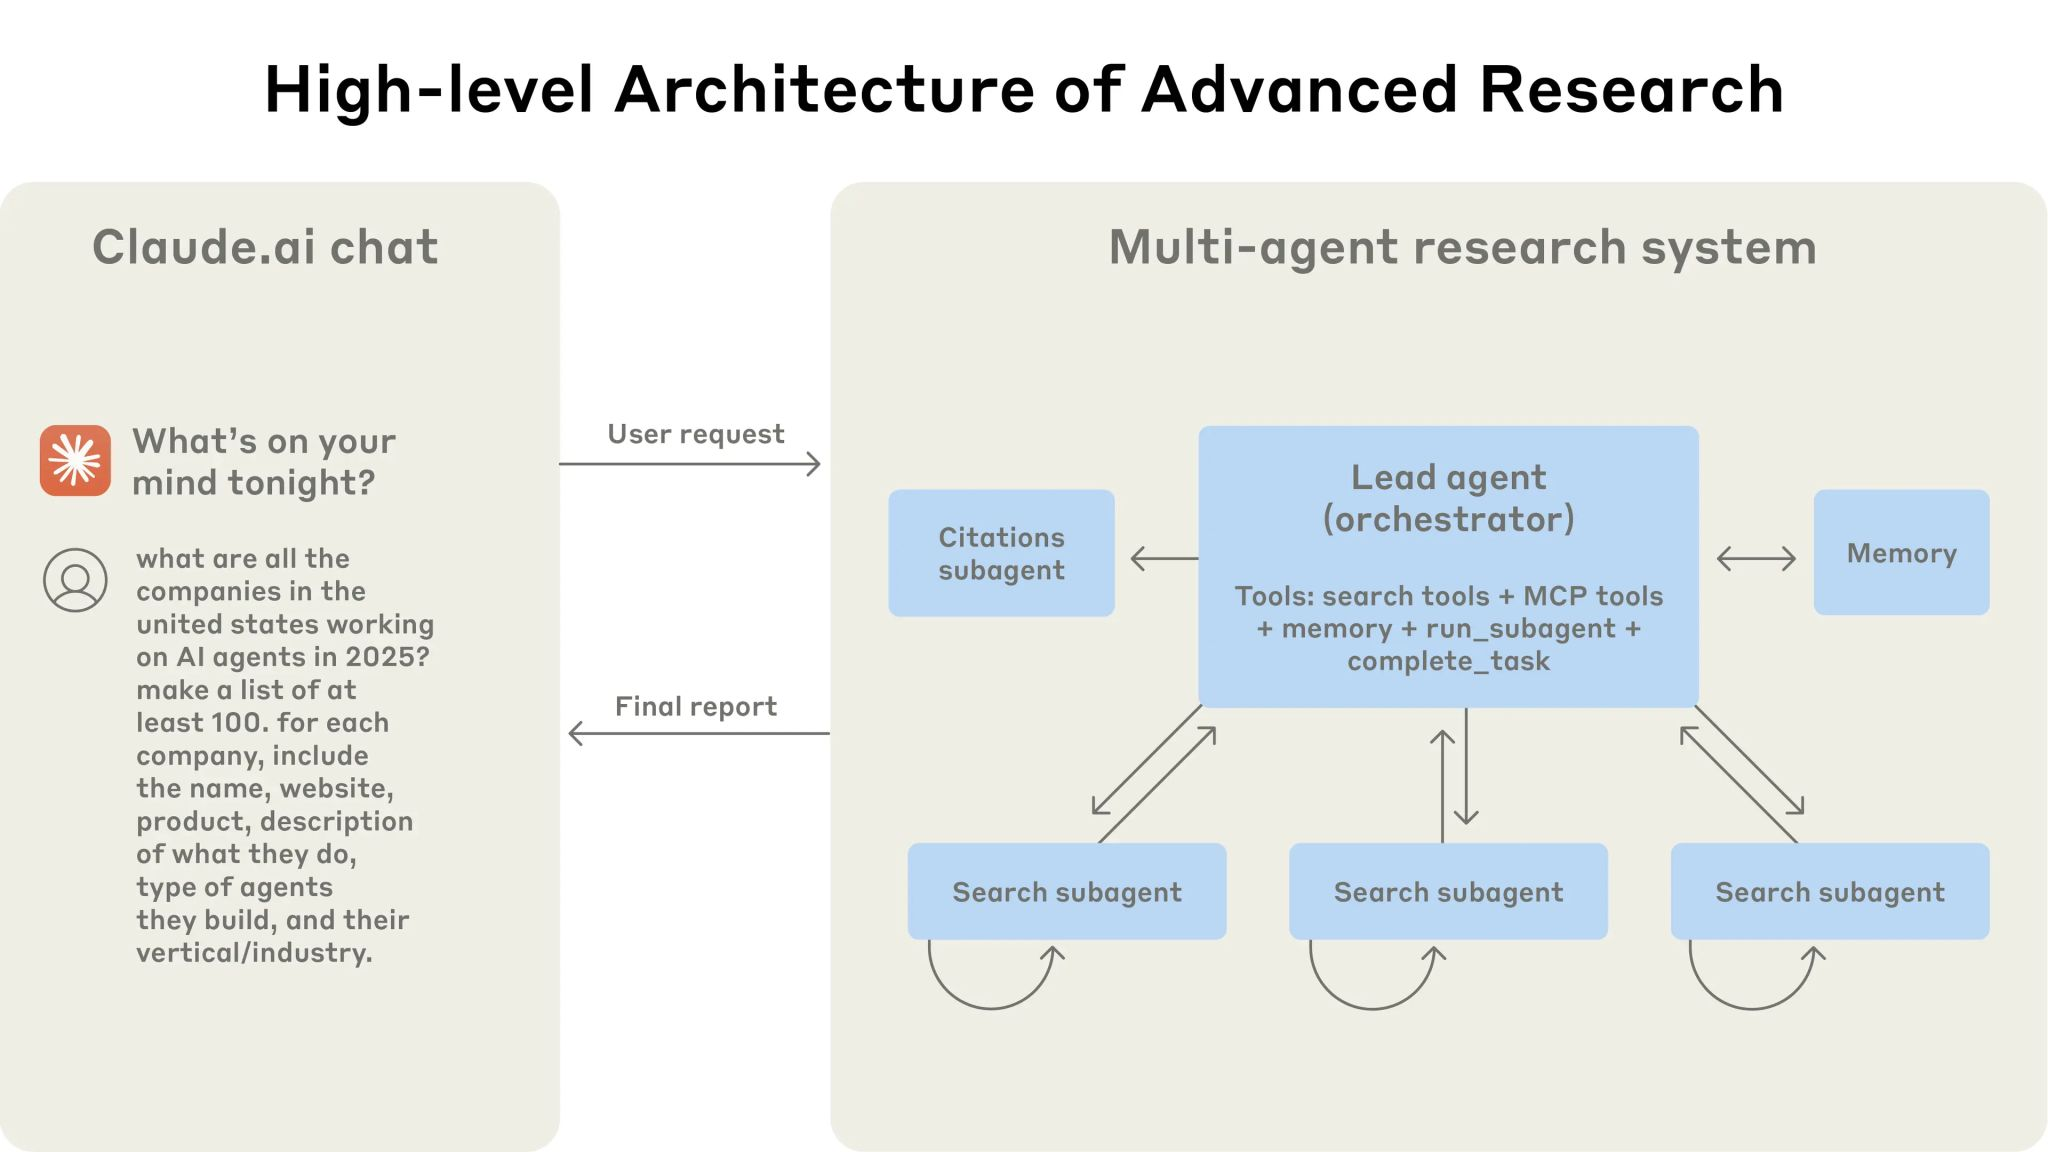
\includegraphics[width=0.8\linewidth,keepaspectratio]{agents5}
	\end{center}
	
{\tiny (Ref: LinkedIn post by Jerry Liu)}

\end{frame}

%%%%%%%%%%%%%%%%%%%%%%%%%%%%%%%%%%%%%%%%%%%%%%%%%%%%%%%%%%%
\begin{frame}[fragile]\frametitle{Process diagram}
	
	\begin{center}
	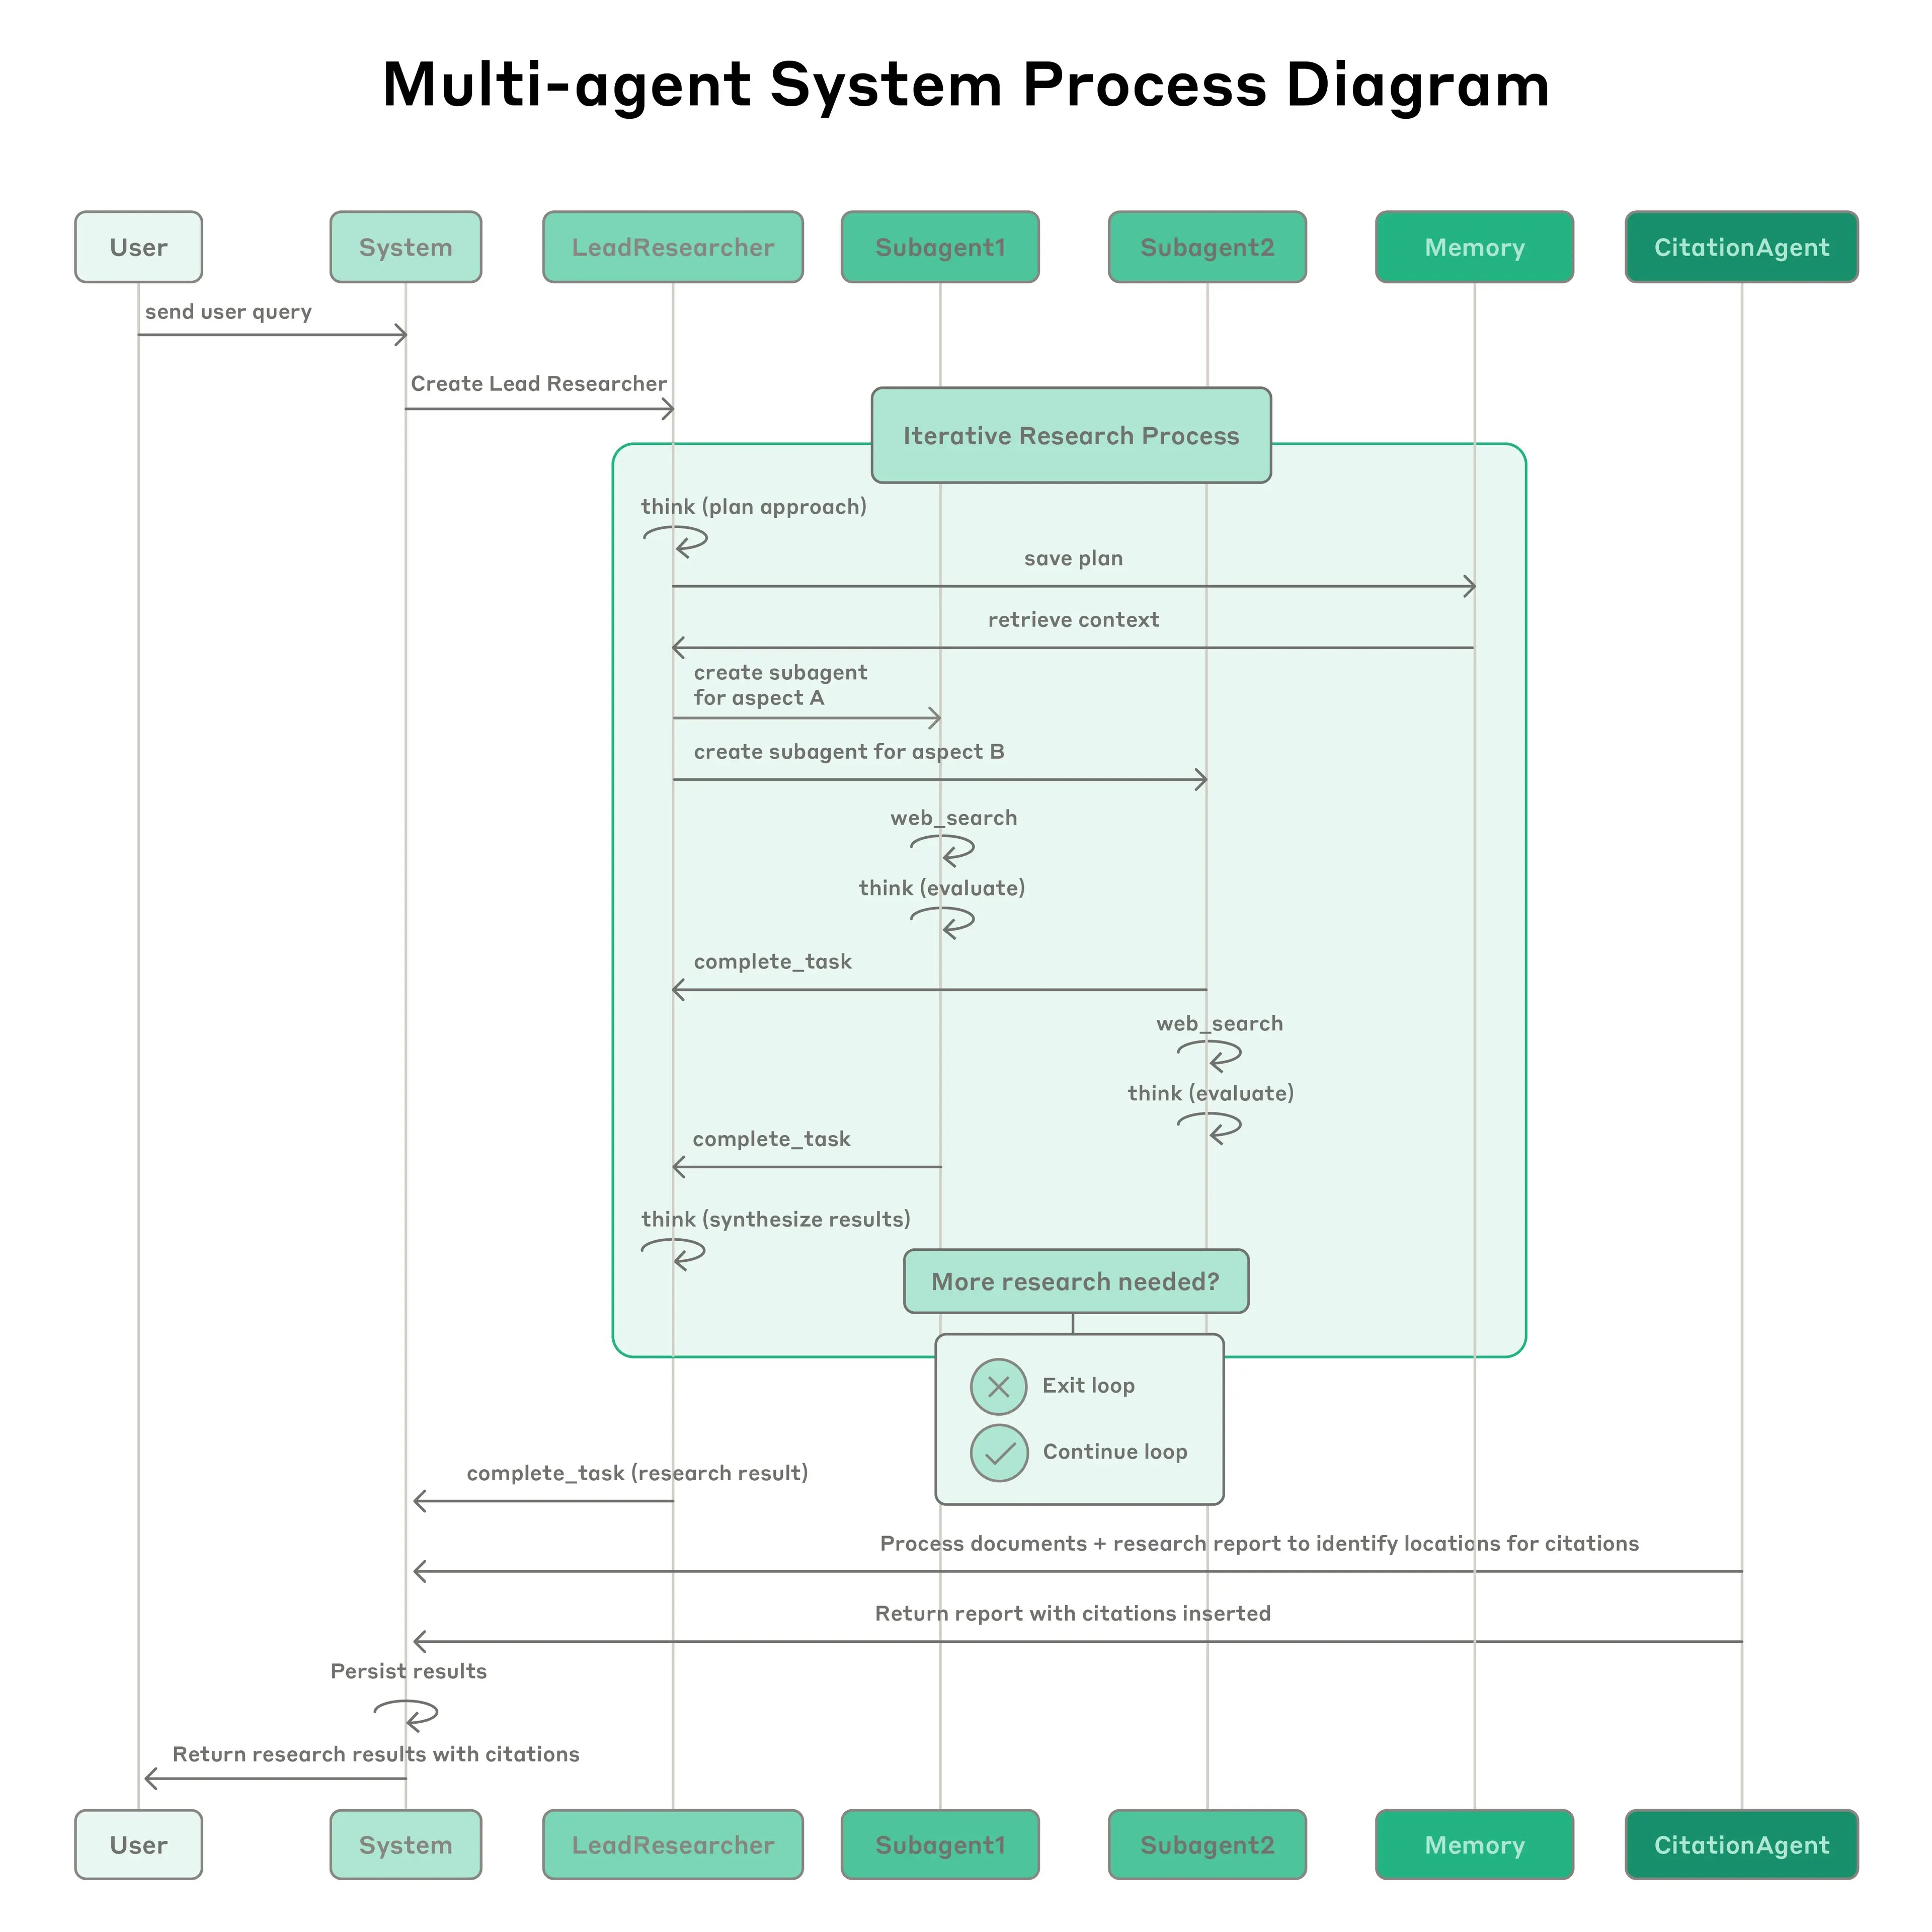
\includegraphics[width=0.6\linewidth,keepaspectratio]{agents6}
	\end{center}
	
{\tiny (Ref: How we built our multi-agent research system - Anthropic)}

\end{frame}

%%%%%%%%%%%%%%%%%%%%%%%%%%%%%%%%%%%%%%%%%%%%%%%%%%%%%%%%%%%
\begin{frame}[fragile]\frametitle{Multi-Agent Research Workflow}
    \begin{itemize}
        \item User query spawns a LeadResearcher agent.
        \item LeadResearcher plans and saves context to Memory.
        \item Specialized subagents are created for subtasks.
        \item Subagents perform web search, analyze results, return findings.
        \item LeadResearcher synthesizes and iterates if needed.
        \item CitationAgent adds source citations to claims.
        \item Final report with citations is returned to user.
    \end{itemize}
\end{frame}

%%%%%%%%%%%%%%%%%%%%%%%%%%%%%%%%%%%%%%%%%%%%%%%%%%%%%%%%%%%
\begin{frame}[fragile]\frametitle{Challenges in Multi-Agent Coordination}
    \begin{itemize}
        \item Early agents over-delegated and created task redundancy.
        \item Coordination complexity grows with agent count.
        \item Prompt engineering was key to guiding agent behavior.
        \item Simulations helped reveal failure modes.
        \item Agents often misused tools or duplicated tasks.
    \end{itemize}
\end{frame}

%%%%%%%%%%%%%%%%%%%%%%%%%%%%%%%%%%%%%%%%%%%%%%%%%%%%%%%%%%%
\begin{frame}[fragile]\frametitle{Effective Prompt Engineering}
    \begin{itemize}
        \item Build mental models to improve prompt quality.
        \item Use simulations to observe and refine behavior.
        \item Prompts guide delegation, scope, and tool use.
        \item Poor task descriptions cause duplication and gaps.
        \item Prompts should scale agent effort to task complexity.
    \end{itemize}
\end{frame}

%%%%%%%%%%%%%%%%%%%%%%%%%%%%%%%%%%%%%%%%%%%%%%%%%%%%%%%%%%%
\begin{frame}[fragile]\frametitle{Optimizing Tool Usage}
    \begin{itemize}
        \item Tool choice is critical-must match user intent.
        \item Agents are taught to assess tool relevance first.
        \item Specialized tools are preferred over generic ones.
        \item Bad tool descriptions can derail agent behavior.
        \item Self-improving agents rewrite flawed tool descriptions.
    \end{itemize}
\end{frame}

%%%%%%%%%%%%%%%%%%%%%%%%%%%%%%%%%%%%%%%%%%%%%%%%%%%%%%%%%%%
\begin{frame}[fragile]\frametitle{Search Strategy and Thinking}
    \begin{itemize}
        \item Begin with broad queries, then narrow focus.
        \item Extended ``thinking'' improves planning and reasoning.
        \item Subagents evaluate results and refine iteratively.
        \item Heuristics guide when to explore vs. go deep.
        \item Avoid verbose or overly specific search queries initially.
    \end{itemize}
\end{frame}

%%%%%%%%%%%%%%%%%%%%%%%%%%%%%%%%%%%%%%%%%%%%%%%%%%%%%%%%%%%
\begin{frame}[fragile]\frametitle{Parallelism and Performance Gains}
    \begin{itemize}
        \item Lead agent spawns subagents in parallel.
        \item Subagents use multiple tools concurrently.
        \item Parallel execution cuts research time drastically.
        \item Enables broad exploration within short timeframes.
        \item Improves system responsiveness for complex queries.
    \end{itemize}
\end{frame}

%%%%%%%%%%%%%%%%%%%%%%%%%%%%%%%%%%%%%%%%%%%%%%%%%%%%%%%%%%%
\begin{frame}[fragile]\frametitle{Reliability in Production Systems}
    \begin{itemize}
        \item Agents must persist state across long tasks.
        \item System supports graceful error recovery and resumption.
        \item Observability helps trace agent failures without logging content.
        \item Debugging focuses on behavior patterns, not just outputs.
        \item Rainbow deployments prevent disruption during updates.
    \end{itemize}
\end{frame}

%%%%%%%%%%%%%%%%%%%%%%%%%%%%%%%%%%%%%%%%%%%%%%%%%%%%%%%%%%%
\begin{frame}[fragile]\frametitle{Sync vs. Async Agent Execution}
    \begin{itemize}
        \item Current systems use synchronous agent execution.
        \item Sync simplifies coordination but slows down progress.
        \item Async allows subagents to act independently.
        \item Adds complexity in managing state and errors.
        \item Anticipated performance gains justify the shift.
    \end{itemize}
\end{frame}

%%%%%%%%%%%%%%%%%%%%%%%%%%%%%%%%%%%%%%%%%%%%%%%%%%%%%%%%%%%
\begin{frame}[fragile]\frametitle{From Prototype to Production}
    \begin{itemize}
        \item Minor bugs can cause cascading behavioral failures.
        \item Agent systems need more engineering than expected.
        \item Testing, iteration, and collaboration are essential.
        \item Guardrails prevent runaway agent behavior.
        \item Final systems must handle edge cases gracefully.
    \end{itemize}
\end{frame}

%%%%%%%%%%%%%%%%%%%%%%%%%%%%%%%%%%%%%%%%%%%%%%%%%%%%%%%%%%%
\begin{frame}[fragile]\frametitle{Impact and User Value}
    \begin{itemize}
        \item Users save days by uncovering hidden connections.
        \item Agents assist in business, healthcare, and debugging.
        \item Multi-agent systems solve complex research tasks.
        \item Careful design makes these systems reliable at scale.
        \item They are transforming how people tackle hard problems.
    \end{itemize}
\end{frame}


%%%%%%%%%%%%%%%%%%%%%%%%%%%%%%%%%%%%%%%%%%%%%%%%%%%%%%%%%%%
\begin{frame}[fragile]\frametitle{Not All Use Cases Need Multi-Agents}
    \begin{itemize}
        \item Some domains require shared context among agents
        \item High interdependencies reduce multi-agent effectiveness
        \item Not every task benefits from parallel agent workflows
    \end{itemize}
\end{frame}

%%%%%%%%%%%%%%%%%%%%%%%%%%%%%%%%%%%%%%%%%%%%%%%%%%%%%%%%%%%
\begin{frame}[fragile]\frametitle{Single vs Multi-Agent Debate}
    \begin{itemize}
        \item Similar point made by Cognition's ``Don't Build Multi-Agents''
        \item Both agree: multi-agents fit a specific class of problems
        \item Focus should be on identifying those right-fit use cases
    \end{itemize}
\end{frame}

%%%%%%%%%%%%%%%%%%%%%%%%%%%%%%%%%%%%%%%%%%%%%%%%%%%%%%%%%%%
\begin{frame}[fragile]\frametitle{Sub-Agents as Tools, Not Peers}
    \begin{itemize}
        \item Claude's system treats sub-agents like tools
        \item No explicit agent-to-agent handoffs
        \item Simplifies control and orchestration
    \end{itemize}
\end{frame}

%%%%%%%%%%%%%%%%%%%%%%%%%%%%%%%%%%%%%%%%%%%%%%%%%%%%%%%%%%%
\begin{frame}[fragile]\frametitle{Agents Improve Tool Interfaces}
    \begin{itemize}
        \item Claude uses a tool testing agent to refine tool descriptions
        \item Agent rewrites unclear interfaces after testing failures
        \item Result: 40\% reduction in task time for future agents
    \end{itemize}
\end{frame}

%%%%%%%%%%%%%%%%%%%%%%%%%%%%%%%%%%%%%%%%%%%%%%%%%%%%%%%%%%%
\begin{frame}[fragile]\frametitle{Self Improving Agents in Practice}
    \begin{itemize}
        \item Tool ergonomics improved through feedback loops
        \item Agents help reduce integration complexity
        \item Smarter interface   fewer downstream errors
    \end{itemize}
\end{frame}

%%%%%%%%%%%%%%%%%%%%%%%%%%%%%%%%%%%%%%%%%%%%%%%%%%%%%%%%%%%
\begin{frame}[fragile]\frametitle{Synchronous Execution   Bottlenecks}
    \begin{itemize}
        \item Claude's agents wait synchronously for sub agent results
        \item Simplifies coordination, but delays execution
        \item Creates sequential bottlenecks in agent chains
    \end{itemize}
\end{frame}

%%%%%%%%%%%%%%%%%%%%%%%%%%%%%%%%%%%%%%%%%%%%%%%%%%%%%%%%%%%
\begin{frame}[fragile]\frametitle{The Case for Async Architectures}
    \begin{itemize}
        \item Event driven models allow async agent execution
        \item Each agent acts as events arrive-faster coordination
        \item Matches design in frameworks like LlamaIndex workflows
    \end{itemize}
\end{frame}

%%%%%%%%%%%%%%%%%%%%%%%%%%%%%%%%%%%%%%%%%%%%%%%%%%%%%%%%%%%
\begin{frame}[fragile]\frametitle{Key Lessons from Claude Research}
    \begin{itemize}
        \item Use multi agent design selectively and purposefully
        \item Let agents optimize tools and interfaces over time
        \item Consider async architectures to eliminate bottlenecks
    \end{itemize}
\end{frame}
